\documentclass[11pt,xcolor=dvipsnames,table]{beamer} %handout %table

% Specify theme
\usetheme{Madrid}
% See deic.uab.es/~iblanes/beamer_gallery/index_by_theme.html for other themes

% Specify base color
\usecolortheme[named=Blue]{structure}
% See http://goo.gl/p0Phn for other colors

% Specify other colors and options as required
\setbeamercolor{alerted text}{fg=Blue}
\setbeamertemplate{items}[square]

\usepackage{graphicx} % Allows including images
\usepackage{booktabs} % Allows the use of \toprule, \midrule and \bottomrule in tables
\usepackage{multirow}
\usepackage{tabularx}
\usepackage{adjustbox}
\usepackage{caption,textcmds}
\usepackage{tikz,qtree,amsmath,bm,xcolor,mathrsfs,amsfonts}
\usepackage{color, colortbl,siunitx,adjustbox}
\usepackage{dcolumn,mathtools}
\usepackage[natbib=true,backend=bibtex,style=authoryear-comp,dashed=false,maxbibnames=99,firstinits=true,maxcitenames=3,url=true,doi=false,isbn=false]{biblatex}
%\usepackage[pdftex,colorlinks=true]{hyperref}
\hypersetup{colorlinks,citecolor=blue,linkcolor=blue,urlcolor=blue}
\DeclareMathOperator*{\argmin}{arg\,min}
\newcolumntype{d}[1]{D{.}{.}{#1}}
\def\E{\text{E}}

\usepackage[natbib=true,backend=bibtex,style=authoryear-comp,dashed=false,maxbibnames=99,firstinits=true,maxcitenames=3,url=true,doi=false,isbn=false]{biblatex}

\DeclareFieldFormat{url}{\url{#1}}
\DeclareFieldFormat[article]{pages}{#1}
\DeclareFieldFormat[inproceedings]{pages}{\lowercase{pp.}#1}
\DeclareFieldFormat[incollection]{pages}{\lowercase{pp.}#1}
\DeclareFieldFormat[article]{volume}{\mkbibbold{#1}}
\DeclareFieldFormat[article]{number}{\mkbibparens{#1}}
\DeclareFieldFormat[article]{title}{\MakeCapital{#1}}
\DeclareFieldFormat[article]{url}{}
\DeclareFieldFormat[book]{url}{}
\DeclareFieldFormat[inbook]{url}{}
\DeclareFieldFormat[incollection]{url}{}
\DeclareFieldFormat[inproceedings]{url}{}
\DeclareFieldFormat[inproceedings]{title}{#1}
\DeclareFieldFormat{shorthandwidth}{#1}
% No dot before number of articles
\usepackage{xpatch}
\xpatchbibmacro{volume+number+eid}{\setunit*{\adddot}}{}{}{}
% Remove In: for an article.
\renewbibmacro{in:}{%
	\ifentrytype{article}{}{%
		\printtext{\bibstring{in}\intitlepunct}}}
% Get rid of months in dates (not sure that this works)
\AtEveryBibitem{\clearfield{month}}
\AtEveryCitekey{\clearfield{month}}
% Title and author information
\title[\textcolor{white}{Probabilistic Hierarchical Forecasting}]{Probabilistic Forecasts for Hierarchical Time Series}
\author[Puwasala Gamakumara]{Candidate:\\Puwasala Gamakumara\\ \medskip \medskip Supervisors:\\  Rob J. Hyndman, George Athanasopoulos,\\Anastasios Panagiotelis }
\institute[]{Department of Econometrics and Business Statistics\\ \medskip Monash University}


\date{May 23, 2019}

\newcommand\tab[1][1cm]{\hspace*{#1}}

\newcounter{saveenumi}
\newcommand{\seti}{\setcounter{saveenumi}{\value{enumi}}}
\newcommand{\conti}{\setcounter{enumi}{\value{saveenumi}}}
\def\PQ{\begin{pmatrix}\bm{P}\\[-0.2cm]\bm{Q}\end{pmatrix}}
\def\bt{\begin{pmatrix}\tilde{\bm{b}}_{t+h}\\[-0.2cm]\tilde{\bm{a}}_{t+h}\end{pmatrix}}
\def\bth{\begin{pmatrix}\tilde{\bm{b}}_{T+h}\\[-0.2cm]\tilde{\bm{a}}_{T+h}\end{pmatrix}}
\def\Naive{Na\"{i}ve\ }
\def\naive{na\"{i}ve\ }

%\begin{adjustbox}{max size={\textwidth}{\textheight}}
%	\includegraphics[#1]{#3}%
%\end{adjustbox}
\resetcounteronoverlays{saveenumi}
\bibliography{References_Pre-submission_review}

\begin{document}

\begin{frame}
\titlepage
\end{frame}

\begin{frame}
\frametitle{Overview} % Table of contents slide, comment this block out to remove it
\tableofcontents % Throughout your presentation, if you choose to use \section{} and \subsection{} commands, these will automatically be printed on this slide as an overview of your presentation
\end{frame}

%\section{Introduction}

%\begin{frame}
%\frametitle[]
%%\frametitle{A first slide}
%
%\begin{center}
%\Huge Introduction
%\end{center}
%\end{frame}




%-------------------%
%\begin{frame}
%	\frametitle{Introduction \textit{Cont..}}
%	\begin{itemize}[<+-| alert@+>]
%		\item Traditional approaches for coherent point forecasts:
%			\begin{itemize}[<+-| alert@+>]
%				\item[$\bullet$] Bottom-up
%				\item[$\bullet$] Top-down
%				\item[$\bullet$] Middle-out
%			\end{itemize}
%		\item Use only part of the information available
%		\item[]
%		\item Point forecast reconciliation \citep{Hyndman2011}
%		\begin{itemize}[<+-| alert@+>]
%			\item[$\bullet$] OLS
%			\item[$\bullet$] MinT \citep{Wickramasuriya2018}
%		\end{itemize}
%		\item[]
%		\item Traditional methods are not reconciliation methods
%%Minimizes the Mean Squared Error of aggregate consistent unbiased point forecasts
%
%	\end{itemize}
%\end{frame}

%-------------------%

%\begin{frame}{Motivation of the study}
%	\begin{itemize}[<+-| alert@+>]
%		\item Importance of probabilistic forecasts in time series \\
%		\item[]
%		\item Probabilistic forecasts of hierarchical time series should reflect the inherent properties of real data. In particular, 
%		\begin{itemize}[<+-| alert@+>]
%			\item[$\star$] Aggregation structure
%			\item[$\star$] Correlation structure
%		\end{itemize}
%		\item Lack of attention on probabilistic forecasting in hierarchical literature
%			\begin{itemize}[<+-| alert@+>]
%				\item[$\bullet$] ``Hierarchical probabilistic forecasting of electricity demand with smart meter data" \citep{BenTaieb2017}
%				\item[$\bullet$]``Reconciliation of probabilistic forecasts with an application to wind power" \citep{Jeon2018}
%		\end{itemize}
%		\item[]
%		\item Extending the ``reconciliation" method into probabilistic framework
%		
%\item[]
%\item \textbf{\color{Maroon}Objective:} Reconciliation of probabilistic forecasts for hierarchical time series such that they preserve the inherent properties of the hierarchical nature\\
%	\end{itemize}
%\end{frame}

%-----------------------------------------

\section{Project 1: Hierarchical Forecast Reconciliation: A Geometric View}

\begin{frame}
\frametitle[]
%\frametitle{A first slide}

\begin{center}
\Huge Project 1: Hierarchical Forecast Reconciliation: A Geometric View
\end{center}
\end{frame}

\begin{frame}[noframenumbering]{Project 1: \textit{Motivation and Contributions}}
	\begin{itemize}[<+-| alert@+>]
			\item \textbf{Example:} 
			\begin{figure}

				\begin{center}
				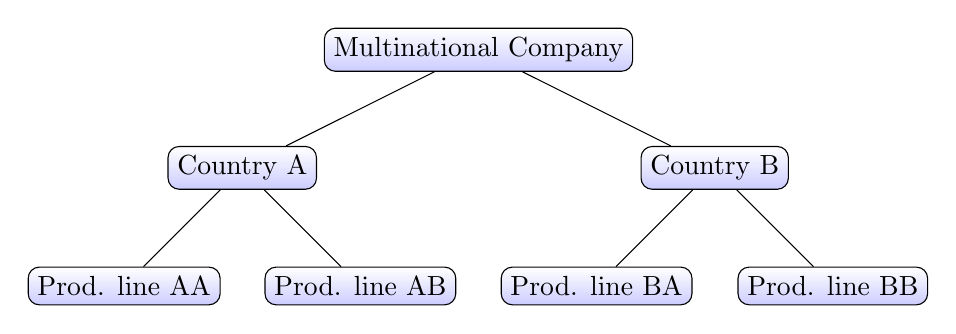
\begin{tikzpicture}[level/.style={sibling distance = 6cm/#1},
every node/.style = {shape=rectangle, rounded corners,
	draw, align=center,
	top color=white, bottom color=blue!20}]
\node {Multinational Company}
child {node {Country A} 
	child {node {Prod. line AA}}
	child {node {Prod. line AB}}
}
child {node {Country B} 
	child {node {Prod. line BA}}
	child {node {Prod. line BB}}
};
\end{tikzpicture}
				\end{center}
			\end{figure}
		\item []
		
		\item \textbf{Hierarchical time series:} A collection of multiple time series that has an inherent aggregation structure. 
		\item Forecasts should add up. We call these \textit{coherent}.
		\item \textbf{\color{Maroon}Contribution:} Provide definitions for coherency and reconciliation of point forecasts in terms of geometric concepts.\\
		
		\end{itemize}
\end{frame}

%\subsection{Notations in hierarchical time series and forecasting}

\begin{frame}{Project 1: \textit{Notations and Preliminaries}}
	\begin{itemize}[<+-| alert@+>]
		\item[] 
			\begin{columns}
          		\column{0.25\linewidth}
             	\centering
             	\begin{figure}
	 				\begin{center}
						\leaf{AA} \leaf{AB} 
						\branch{2}{A}
						\leaf{BA} \leaf{BB}
						\branch{2}{B}
						\branch{2}{Tot}
						\qobitree
					\end{center}
				\end{figure}

     			\column{0.70\linewidth}
        			\begin{itemize}[<+-| alert@+>]
						\item[]$\bm{y}_t = [y_{Tot,t},y_{A,t}, y_{B,t},y_{AA,t}, y_{AB,t}, y_{BA,t}, y_{BB,t}]^T$	
						\item[]$\bm{b}_t = [y_{AA,t}, y_{AB,t}, y_{BA,t}, y_{BB,t}]^T$	
						\item[]$m = 4$
						\item[]$n = 7$
						\item[]${\bm S}=\begin{pmatrix} 1 &1 &1 &1 \\1 &1 &0 &0 \\0 &0 &1 &1 \\ &{\bm I_{4\times 4}}
						\end{pmatrix}  $
	    			\end{itemize}	
       		\end{columns} 
		\item Due to the aggregation nature of the hierarchy we have, 
$$\color{Maroon} \bm{y}_t = \bm{Sb}_t.$$
		\item[]
		\begin{block}{Coherent subspace}
			The $m$-dimensional linear subspace $\mathfrak{s}\subset \mathbb{R}^n$ that is spanned by the columns of $\bm{S}$, i.e.\ $\mathfrak{s}=\text{span}(\bm{S})$, is defined as the \emph{coherent space}.
		\end{block}
	\end{itemize}    
\end{frame}

%-------------------

\begin{frame}{Project 1: \textit{Coherent forecasts}}
\begin{itemize}
	\item[] 		
%	\centering
	\begin{center}
	\vspace{-1.5cm}
	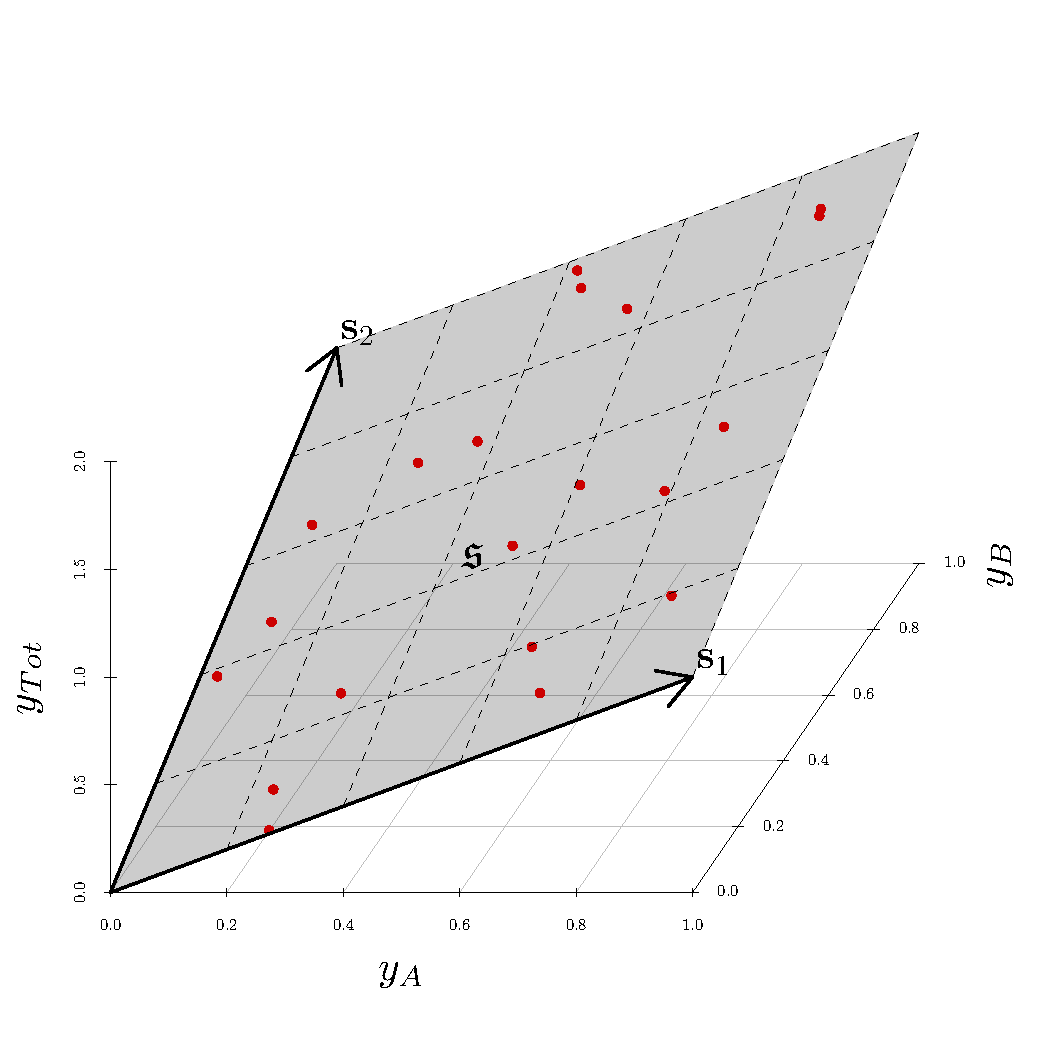
\includegraphics[scale=0.40]{Figs/3D_hierarchy}
	\end{center}
	\item Three dimensional hierarchy, $y_{Tot} = y_A + y_B$.
	\item $\vec{s}_1 = (1,1,0)'$ and $\vec{s}_2 = (1, 0, 1)'$ form a basis for $\mathfrak{s}$.
\end{itemize}    
\end{frame}


%--------------------

%\begin{frame}{Point forecasts: \textit{Reconciliation}}
%\begin{itemize}[<+-| alert@+>]
%	\item[]
%	\begin{center}
%		\begin{block}{}
%			\begin{table}
%				\small
%				\centering %\setstretch{1.5}
%				\begin{tabular}{lc}
%					\toprule
%					\textbf{Method} & \textbf{$\bm{G}$} \\
%					\midrule
%					BU             & $\left(\bm{0}_{m\times n-m}~\bm{I}_{m\times m}\right)$\\
%					OLS             &
%					$\left(\bm{S}'\bm{S}\right)^{-1}{\bm S'}$  \\
%					WLS    &
%					$\left(\bm{S}'\bm{\hat{W}}_{T+1}^{wls}\bm{S}\right)^{-1}\bm{S}'\bm{\hat{W}}_{T+1}^{wls}$ \\
%					MinT(Shrink)    &
%					$\left(\bm{S}'\bm{\hat{W}}_{T+1}^{shr}\bm{S}\right)^{-1}\bm{S}'\bm{\hat{W}}_{T+1}^{shr}$ \\
%					\bottomrule
%				\end{tabular}
%			\end{table}
%		\end{block}
%		\begin{table}
%			\small
%			\centering %\setstretch{1.5}
%			\begin{tabular}{lll}
%				\toprule
%				$\bm{\hat{W}}_{T+1}^{shr}$ & = & $\tau\text{Diag}(\bm{\hat{W}}_{T+1}^{sam}) + (1-\tau)\bm{\hat{W}}_{T+1}^{sam}$\\
%				$\bm{\hat{W}}_{T+1}^{wls}$ & = & $\text{Diag}(\bm{\hat{W}}_{T+1}^{shr})$\\
%				\bottomrule
%			\end{tabular}
%		\end{table}
%	\end{center}
%	
%	
%	
%	
%\end{itemize}
%\end{frame}


\begin{frame}{Project 1: \textit{Point forecast reconciliation}}
\begin{itemize}[<+-| alert@+>]
	\item Let $\hat{\bm y}\in\mathbb{R}^n$ be an incoherent forecast and $g(.)$ be a function $g:\mathbb{R}^n\rightarrow\mathbb{R}^m$.
	\begin{definition} 
		{\bf Point forecasts} $\tilde{\bm y}$ are reconciled with respect to $g(.)$ iff 
		\begin{equation*}
		\tilde{\bm y}={\bm S}g(\hat{\bm y})
		\end{equation*}
	\end{definition}
	\item[]
	\item If $g(.)$ is linear,
		\begin{equation*}
			\color{Maroon}\tilde{\bm y}_{T+h} = \bm{SG}\hat{\bm y}_{T+h}.
		\end{equation*}
	\item Single level approaches:
	\begin{itemize}[<+-| alert@+>]
		\item Bottom-up: $\color{Purple}\bm{G}=\begin{pmatrix}
		\bm{0}_{(m \times n-m)} & \bm{I}_m
		\end{pmatrix}$
		\item Top-down: $\color{Purple}\bm{G}=\begin{pmatrix}
		\bm{p} & \bm{0}_{(m \times n-1)}
		\end{pmatrix}$
	\end{itemize}	
 		
\end{itemize}    
\end{frame}


%-------------------

%\begin{frame}{Project 1: \textit{Point forecast reconciliation}}
%\begin{itemize}[<+-| alert@+>]
%	\item[] 
%	\resizebox{\linewidth}{!}{	
%	% Created by tikzDevice version 0.12 on 2019-04-24 17:20:56
% !TEX encoding = UTF-8 Unicode
\begin{tikzpicture}[x=1pt,y=1pt]
\definecolor{fillColor}{RGB}{255,255,255}
\path[use as bounding box,fill=fillColor,fill opacity=0.00] (0,0) rectangle (505.89,361.35);
\begin{scope}
\path[clip] ( 49.20, 61.20) rectangle (480.69,312.15);
\definecolor{drawColor}{RGB}{0,0,0}

\path[draw=drawColor,line width= 0.4pt,line join=round,line cap=round] ( 88.68, 49.37) --
	( 88.68,302.86);

\path[draw=drawColor,line width= 0.4pt,line join=round,line cap=round] (  0.00, 91.62) --
	(505.89, 91.62);

\path[draw=drawColor,line width= 1.2pt,line join=round,line cap=round] ( 88.68, 91.62) -- (417.71,165.55);

\path[draw=drawColor,line width= 1.2pt,line join=round,line cap=round] (404.42,153.31) --
	(417.71,165.55) --
	(400.46,170.93);

\node[text=drawColor,anchor=base west,inner sep=0pt, outer sep=0pt, scale=  1.00] at (423.71,163.26) {{\Large ${\bm S}$}};

\node[text=drawColor,anchor=base,inner sep=0pt, outer sep=0pt, scale=  1.00] at (276.70,112.53) {{\huge $\mathfrak{s}$}};

\path[draw=drawColor,line width= 1.2pt,line join=round,line cap=round] ( 88.68, 91.62) -- (182.69,260.61);

\path[draw=drawColor,line width= 1.2pt,line join=round,line cap=round] (182.98,242.54) --
	(182.69,260.61) --
	(167.19,251.33);

\node[text=drawColor,anchor=base,inner sep=0pt, outer sep=0pt, scale=  1.00] at (182.69,266.61) {{\Large ${\bm R}$}};

\path[draw=drawColor,line width= 0.4pt,dash pattern=on 4pt off 4pt ,line join=round,line cap=round] (108.22,  0.00) --
	(276.70,302.86);
\definecolor{drawColor}{RGB}{0,0,255}
\definecolor{fillColor}{RGB}{0,0,255}

\path[draw=drawColor,line width= 0.4pt,line join=round,line cap=round,fill=fillColor] (229.69,218.36) circle (  3.00);
\definecolor{drawColor}{RGB}{0,0,0}

\node[text=drawColor,anchor=base,inner sep=0pt, outer sep=0pt, scale=  1.00] at (229.69,236.36) {{\huge $\color{blue}{\hat{\bm{y}}}$}};

\node[text=drawColor,anchor=base west,inner sep=0pt, outer sep=0pt, scale=  1.00] at (212.19,173.82) {{\huge ${\color{blue} s\circ g}$}};
\definecolor{drawColor}{RGB}{255,0,0}
\definecolor{fillColor}{RGB}{255,0,0}

\path[draw=drawColor,line width= 0.4pt,line join=round,line cap=round,fill=fillColor] (169.26,109.72) circle (  3.00);
\definecolor{drawColor}{RGB}{0,0,0}

\node[text=drawColor,anchor=base,inner sep=0pt, outer sep=0pt, scale=  1.00] at (169.26, 85.99) {{\huge $\color{red}{\tilde{\bm{y}}}$}};
\definecolor{drawColor}{RGB}{0,0,255}

\path[draw=drawColor,line width= 0.4pt,line join=round,line cap=round] (229.69,218.36) -- (169.26,109.72);

\path[draw=drawColor,line width= 0.4pt,line join=round,line cap=round] (168.97,127.79) --
	(169.26,109.72) --
	(184.76,119.01);
\end{scope}
\end{tikzpicture}

%}
%\end{itemize}    
%\end{frame}


%-------------------

\begin{frame}{Project 1: \textit{Point forecast reconciliation - OLS}}
\begin{itemize}[<+-| alert@+>]
	\item[] $ \color{Maroon} \bm{SG} = \bm{S} \left(\bm{S}'\bm{S}\right)^{-1}{\bm S'}$ \citep{Hyndman2011}
	\item[]
	\vspace{-6.3cm}
	\resizebox{\linewidth}{!}{	
		% Created by tikzDevice version 0.12 on 2019-04-26 17:19:46
% !TEX encoding = UTF-8 Unicode
\begin{tikzpicture}[x=1pt,y=1pt]
\definecolor{fillColor}{RGB}{255,255,255}
\path[use as bounding box,fill=fillColor,fill opacity=0.00] (0,0) rectangle (289.08,505.89);
\begin{scope}
\path[clip] ( 49.20, 61.20) rectangle (263.88,456.69);
\definecolor{drawColor}{RGB}{0,0,0}

\path[draw=drawColor,line width= 0.4pt,line join=round,line cap=round] ( 68.84,130.32) --
	( 68.84,317.41);

\path[draw=drawColor,line width= 0.4pt,line join=round,line cap=round] ( 22.07,177.10) --
	(209.16,177.10);

\path[draw=drawColor,line width= 1.2pt,line join=round,line cap=round] ( 68.84,177.10) -- (232.54,258.95);

\path[draw=drawColor,line width= 1.2pt,line join=round,line cap=round] (222.59,243.87) --
	(232.54,258.95) --
	(214.51,260.03);

\node[text=drawColor,anchor=base west,inner sep=0pt, outer sep=0pt, scale=  1.00] at (238.54,256.65) {{\large $\mathfrak{s}$}};
\definecolor{drawColor}{RGB}{0,0,255}
\definecolor{fillColor}{RGB}{0,0,255}

\path[draw=drawColor,line width= 0.4pt,line join=round,line cap=round,fill=fillColor] (139.00,317.41) circle (  3.00);
\definecolor{drawColor}{RGB}{0,0,0}

\node[text=drawColor,anchor=base,inner sep=0pt, outer sep=0pt, scale=  1.00] at (139.00,335.41) {{\large $\color{blue}{\hat{\bm{y}}}$}};
\definecolor{drawColor}{RGB}{255,0,0}
\definecolor{fillColor}{RGB}{255,0,0}

\path[draw=drawColor,line width= 0.4pt,line join=round,line cap=round,fill=fillColor] (181.09,233.22) circle (  3.00);
\definecolor{drawColor}{RGB}{0,0,0}

\node[text=drawColor,anchor=base,inner sep=0pt, outer sep=0pt, scale=  1.00] at (181.09,209.48) {{\large $\color{red}{\tilde{\bm{y}}}$}};
\definecolor{drawColor}{RGB}{0,0,255}

\path[draw=drawColor,line width= 0.4pt,line join=round,line cap=round] (139.00,317.41) -- (181.09,233.22);

\path[draw=drawColor,line width= 0.4pt,line join=round,line cap=round] (166.02,243.18) --
	(181.09,233.22) --
	(182.18,251.26);
\definecolor{drawColor}{RGB}{0,0,0}

\path[draw=drawColor,line width= 0.4pt,dash pattern=on 4pt off 4pt ,line join=round,line cap=round] (139.00,317.41) -- (108.93,197.14);

\path[draw=drawColor,line width= 0.4pt,dash pattern=on 4pt off 4pt ,line join=round,line cap=round] (103.96,214.51) --
	(108.93,197.14) --
	(121.49,210.13);
\definecolor{fillColor}{RGB}{0,0,0}

\path[draw=drawColor,line width= 0.4pt,line join=round,line cap=round,fill=fillColor] (108.93,197.14) circle (  3.00);

\node[text=drawColor,anchor=base,inner sep=0pt, outer sep=0pt, scale=  1.00] at (108.93,173.40) {{\large $\color{black}{{\bm{y}}}$}};
\end{scope}
\end{tikzpicture}

	}
\end{itemize}    
\end{frame}


%-------------------

\begin{frame}{Project 1: \textit{Point forecast reconciliation - MinT}}
\begin{itemize}[<+-| alert@+>]
	\item Minimises the trace of mean squared reconciled forecast errors \citep{Wickramasuriya2018}.
	$$ \color{Maroon} \bm{SG} = \bm{S} \left(\bm{S}'\bm{W}^{-1}_{T+h}\bm{S}\right)^{-1}{\bm S'}\bm{W}^{-1}_{T+h}$$ 
	\item \textbf{Geometry}
  	\begin{itemize}[<+-| alert@+>]
  	\item Consider the covariance matrix $\bm{W}_{T+h}$ of ${\bm y}_{T+h}-\hat{\bm{y}}_{T+h}$.

	\item This can be estimated using in-sample forecast errors.
		\begin{equation*}
		\hat{\bm{W}}_{T+h}=\sum\limits_{t=1}^T ({\bm y}_{t}-\hat{\bm{y}}_{t})({\bm y}_{t}-\hat{\bm{y}}_{t})'
		\end{equation*}
	\pause
	\item This provides information about the likely direction of the largest error variance.
	\pause
	\item Projecting along this direction is more likely to result in reconciled forecasts that are closer to the target.

  \end{itemize}\end{itemize}    
\end{frame}


%-------------------

\begin{frame}{Project 1: \textit{Point forecast reconciliation - MinT}}
\begin{itemize}[<+-| alert@+>]
	\item[] $ \color{Maroon} \bm{SG} = \bm{S} \left(\bm{S}'\bm{W}^{-1}_{T+h}\bm{S}\right)^{-1}{\bm S'}\bm{W}^{-1}_{T+h}$ 
	\tiny
	\resizebox{\linewidth}{!}{
		\begin{overprint}
			\onslide<+|handout:0>
			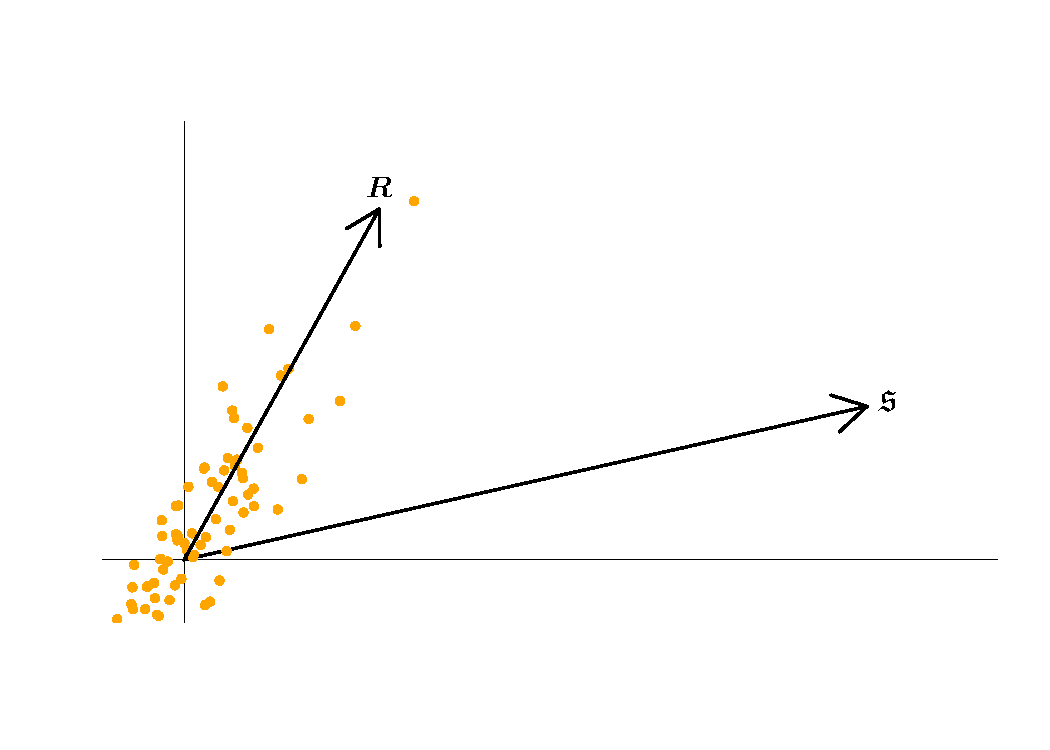
\includegraphics[scale=0.55]{Figs/MinT_justif/Error_dir.pdf}
			\onslide<+|handout:0>
			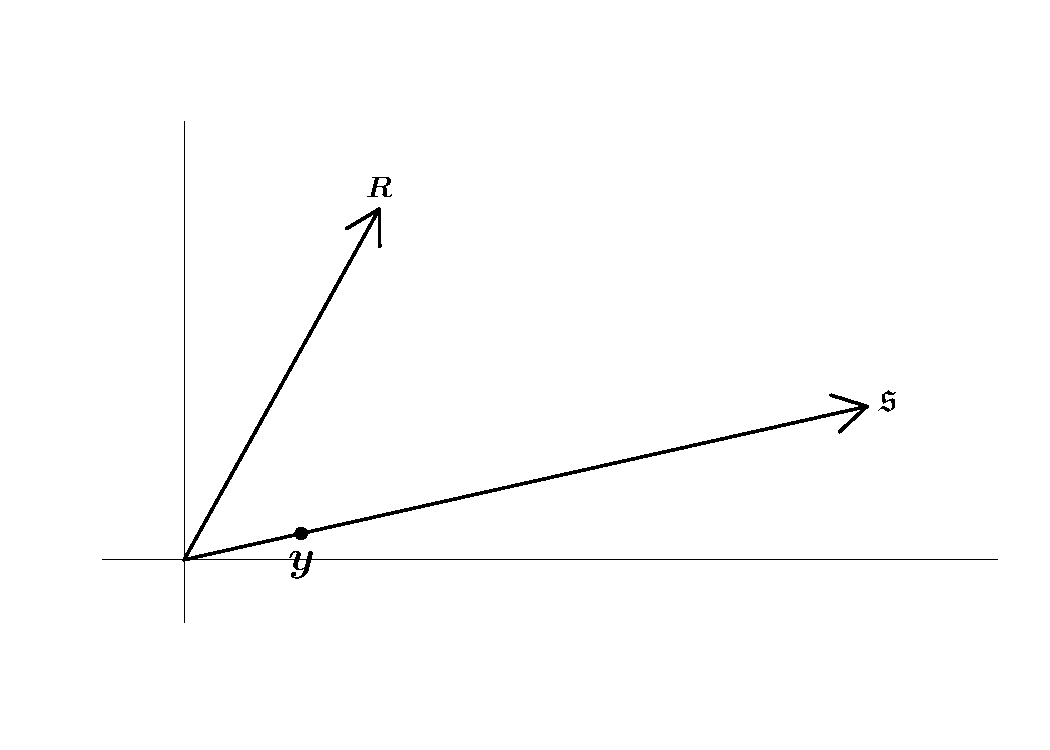
\includegraphics[scale=0.55]{Figs/MinT_justif/Target.pdf}
			\onslide<+|handout:0>
			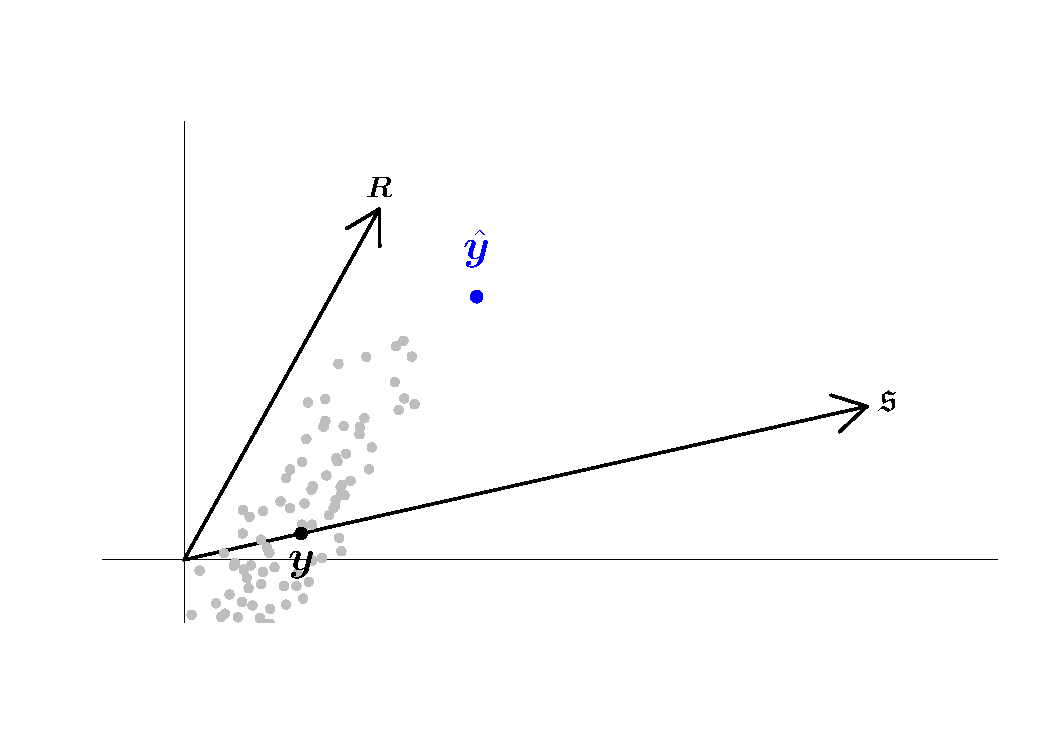
\includegraphics[scale=0.55]{Figs/MinT_justif/SampleEstimates.pdf}
			\onslide<+|handout:0>
			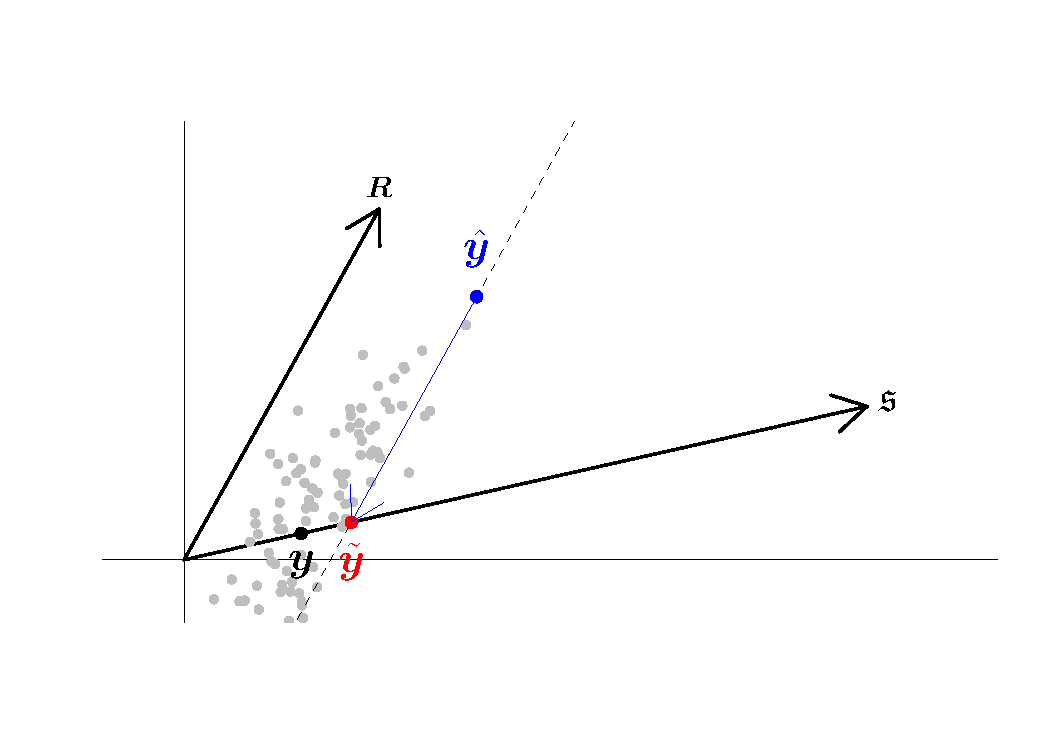
\includegraphics[scale=0.55]{Figs/MinT_justif/ObliqueProjection.pdf}
		\end{overprint}	
}
\end{itemize}    
\end{frame}



%-------------------

\begin{frame}{Project 1: \textit{Why projections?}}
\begin{itemize}[<+-| alert@+>]
	\item Projections onto the coherent subspace preserve unbiasedness.
	\item[]
	\item What if the incoherent forecasts are biased?
	\item[]
	\item Can we bias correct and proceed with projections? 
	\item[] We investigate this further.
\end{itemize}    
\end{frame}

\section{Project 2: Probabilistic Forecasts for Hierarchical Time Series}

\begin{frame}
\frametitle[]
%\frametitle{A first slide}

\begin{center}
	\Huge Project 2: Probabilistic Forecasts for Hierarchical Time Series
\end{center}
\end{frame}

%-------------------

\subsection{Part 1: Definitions and A Parametric Approach}

\begin{frame}[noframenumbering]
\frametitle[]
%\frametitle{A first slide}

\begin{center}
	\Huge Part 1: Definitions and A Parametric Approach
\end{center}
\end{frame}

%-------------------


\begin{frame}[noframenumbering]{Project 2: \textit{Motivation and Contributions}}
\begin{itemize}[<+-| alert@+>]
			\item Probabilistic forecasts should reflect the inherent properties of real data. In particular, 
			\begin{itemize}[<+-| alert@+>]
				\item[$\star$] Aggregation structure
				\item[$\star$] Correlation structure
			\end{itemize}
			\item Lack of attention
				\begin{itemize}[<+-| alert@+>]
					\item[$\bullet$] \citet{BenTaieb2017}
					\item[$\bullet$] \citet{Jeon2018}
			\end{itemize}
		\item Extending ``reconciliation" into a probabilistic framework.
		\item[]
					
	\item \textbf{\color{Maroon}Contributions:} 
	\begin{enumerate}
		\item Provide definitions for coherency and reconciliation for probabilistic forecasts.
		\item[]
		\item A parametric framework for probabilistic forecast reconciliation.
		\item[]
		\item A non-parametric framework for probabilistic forecast reconciliation.
	\end{enumerate}	
	\item[]
	
\end{itemize}    
\end{frame}


%-------------------
%\begin{frame}{Project 2: \textit{Coherent point forecasts}}
%\begin{itemize}[<+-| alert@+>]
%		\item[]
%		\begin{block}{Definition 2: Probabilistic forecasts reconciliation}
%		Let $\mathcal{A}$ be a subset\footnote{Strictly speaking $\mathcal{A}$ is a Borel set} of $\mathfrak{s}$ and let $\mathcal{B}$ be all points in $\mathbb{R}^n$ that are mapped onto $\mathcal{A}$ after pre-multiplication by $\bm{S}\bm{G}$. Letting $\hat{\nu}$ be a base probabilistic forecast for the full hierarchy, the coherent measure $\tilde{\nu}$ reconciles $\hat{\nu}$ if $\tilde{\nu}(\mathcal{A})=\hat{\nu}(\mathcal{B})$ for all $\mathcal{A}$.
%	\end{block}
%	
%\end{itemize}    
%\end{frame}

  \begin{frame}{Project 2: \textit{Coherent probabilistic forecasts}}
Let $(\mathbb{R}^m,\mathcal{F}_{\mathbb{R}^m},\nu)$ and $(\mathfrak{s},\mathcal{F}_{\mathfrak{s}},\mu)$ be probability triples on $m$-dimensional space and the coherent subspace respectively.
\begin{definition}
	The probability measure $\mu$ is coherent if
	\begin{equation*}
	\nu(\mathcal{B})=\mu(s(\mathcal{B}))\quad\forall\mathcal{B}\in \mathcal{F}_{\mathbb{R}_m}
	\end{equation*} 
\end{definition}
where $s(\mathcal{B})$ is the image of $\mathcal{B}$ under premultiplication by ${\bm S}$
\end{frame}
%-------------------

\begin{frame}{Project 2: \textit{Reconciled Probabilistic Forecast}}
Let $g:\mathbb{R}^n\rightarrow\mathbb{R}^m$ be a function.  Then 
\begin{definition}
	The probability triple $\left(\mathfrak{s},\mathcal{F}_{\mathfrak{s}},\tilde{\nu}\right)$ reconciles the probability triple $\left(\mathbb{R}^n,\mathcal{F}_{\mathbb{R}^n},\hat{\nu}\right)$ with with respect to $g$ iff
	\begin{equation*}
	\tilde{\nu}(s(\mathcal{B}))=\nu(\mathcal{B})=\hat{\nu}(g^{-1}(\mathcal{B}))\quad\forall \mathcal{B}\in\mathcal{F}_{\mathbb{R}_m}
	\end{equation*}
\end{definition}
where $g^{-1}$ is the pre-image of $g$.
\end{frame}

%--------------------

\begin{frame}{Project 2: \textit{Geometry}}
\begin{itemize}
	\item[]
	\vspace{-0.5cm}
	\centering
	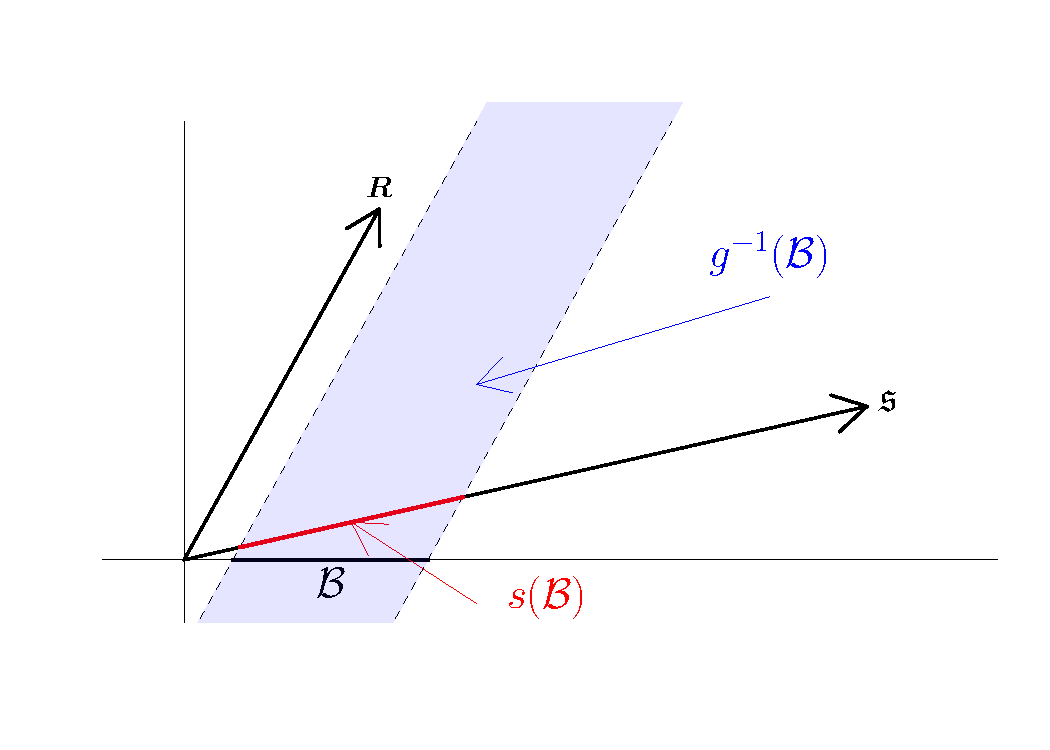
\includegraphics[scale=0.5]{Figs/probforerec_schematic.pdf}
	\item[]\begin{equation*}
	\tilde{\nu}(s(\mathcal{B}))=\hat{\nu}(g^{-1}(\mathcal{B}))\quad\forall \mathcal{B}\in\mathcal{F}_{\mathbb{R}_m}
	\end{equation*} 
\end{itemize}    
\end{frame}


%-------------------

  \begin{frame}{Project 2: \textit{Analytically}}
If we have an unreconciled density the reconciled density can be obtained by linear transformations and marginalisation.
\begin{align*}
\mbox{Pr}(\hat{\bm{y}}\in g^{-1}(\mathcal{B}))&=\int\limits_{g^{-1}(\mathcal{B})}f(\hat{\bm{y}})d\hat{\bm{y}}\\
&=\int\limits_{\mathcal{B}}\int f(\bm{S}\tilde{\bm{b}}+\bm{R}\tilde{\bm{a}})|\left(\bm{S}~\bm{R}\right)|d\tilde{\bm{a}}d\tilde{\bm{b}}\\
&=\mbox{Pr}(\tilde{\bm{b}}\in \mathcal{B})
\end{align*}
\end{frame}

%-------------------


%------------------------



\begin{frame}{Project 2: \textit{Assuming Gaussian distribution}} \hyperlink{GaussianFramework}{\hypertarget{backtoGaussianFramework}{\beamerbutton{A1}}} 
\begin{itemize}[<+-| alert@+>]
	\item Let $\mathscr{N}(\hat{\bm{y}}_{T+h}, \bm{W}_{T+h})$ be an incoherent forecast distribution at time $T+h$
	where $\hat{\bm{y}}_{T+h}$ is the incoherent mean and ${\bm{W}}_{T+h} =E_{\bm{y}_{T+h}}[(\bm{y}_{T+h}-\hat{\bm{y}}_{T+h})(\bm{y}_{T+h}-\hat{\bm{y}}_{T+h})^T|\mathcal{I}_{T}]$ is the incoherent variance 
	%\item Gaussian densities are closed under affine transformation and marginalization
	\item The reconciled Gaussian distribution is given by, 
	$$\color{Maroon}\mathscr{N}(\bm{SG}\bm{\hat{y}}_{T+h},~ \bm{SG}{\bm{W}}_{T+h}\bm{G}'\bm{S}')$$
	
	\item ${\bm G}=\left(\bm{S}'\bm{W}_{T+h}^{-1}\bm{S}\right)^{-1}{\bm S'}\bm{W}_{T+h}^{-1}$ minimizes the energy score in the limiting case
%	\hyperlink{ScoringRules}{\hypertarget{backtoScoringRule}{\beamerbutton{A1}}} 
	\item Simulation study evidence for improved predictive performance in reconciled Gaussian forecast distributions.	
	
\end{itemize}    

\end{frame}

%------------------------

\begin{frame}{Project 2: \textit{For elliptical distributions}}
Consider the case where the base and true predictive distributions are elliptical.
\begin{theorem}
	There exists a matrix $\bm{G}$ such that the true predictive distribution can be recovered by linear reconciliation.
\end{theorem}
This follows from the closure property of elliptical distributions under affine transformations and marginalisation.  
\end{frame}

%-----------------------

 \begin{frame}{Project 2: \textit{Evaluation}}
\begin{itemize}[<+-| alert@+>]
	\item Scoring rules can be used to evaluate probabilistic forecasts 		\hyperlink{ScoringRules}{\hypertarget{backtoScoringRule}{\beamerbutton{A2}}} 
	\pause
	\begin{itemize}
		\item Log Score
		\item Energy Score
		\item Variogram score

	\end{itemize}
	\item[]
	\pause
	\item We may want to compare
	\begin{itemize}
		\item Coherent vs Incoherent
		\item Coherent vs Coherent
	\end{itemize}
\end{itemize}
\end{frame}

%---------------------
\begin{frame}{Project 2: \textit{Evaluation - Coherent vs Incoherent}}
When using log score
\begin{theorem}
Let $f(\bm{y})$ be the true predictive density (on $\mathfrak{s}$) and $LS$ be the (negatively-oriented) log score.  Then there exists an unreconciled density  $\hat{f}(\bm{y})$ on $\mathbb{R}^n$ such that
\begin{equation*}
E_{\bm y}\left[LS(\hat{f},\bm{y})\right]<E_{\bm y}\left[LS(f,\bm{y})\right]
\end{equation*}
\end{theorem}
The log score is not proper {\bf in this context}.
\end{frame}


\begin{frame}[noframenumbering]{Today's talk}
\begin{itemize}[<+-| alert@+>]
	\item A non-parametric bootstrap approach for probabilistic forecast reconciliation.
	\item[]
	\item Hierarchical forecasts for macroeconomic variables - An application to Australian GDP.
\end{itemize}    
\end{frame}

%-----------------------

%%------------------------
\subsection{Part 2: A Non-parametric Bootstrap Approach }

\begin{frame}
\frametitle[]
%\frametitle{A first slide}

\begin{center}
\Huge Part 2: A non-parametric bootstrap approach for probabilistic forecast reconciliation
\end{center}
\end{frame}

%------------------------
\begin{frame}[noframenumbering]{Probabilistic forecast reconciliation: Non-parametric approach}
\begin{itemize}[<+-| alert@+>]
	\item [$\bullet$] Often parametric densities are unavailable but we can simulate a sample from the predictive distribution.
	\item[]
	\item [$\bullet$] Suppose $\hat{\bm y}^{[1]}_{T+h},...,\hat{\bm y}^{[J]}_{T+h}$ is a sample from the incoherent predictive distribution.
	\item[]
	\item [$\bullet$] Then setting $\tilde{\bm y}^{[j]}_{T+h}=\bm{SG}\hat{\bm y}^{[j]}_{T+h}$ produces a sample from the reconciled predictive distribution with respect to $\bm{G}$.
\end{itemize}    
\end{frame}

%-----------------------


\begin{frame}{A Non-parametric approach}
\begin{enumerate}[<+-| alert@+>]
\item Fit univariate models at each node using data up to time $T$.
\item[]
\item Let $\bm{\Gamma}_{(T \times n)}=(\bm{e}_1,\bm{e}_2,\dots,\bm{e}_T)'$ be a matrix of in-sample residuals\\
where $\bm{e}_t=\bm{y}_t-\hat{\bm{y}}_t$. 
\item[]
\item Let $\bm{\Gamma}^b_{(H \times n)} = (\bm{e}^b_1,...,\bm{e}^b_H)'$ be a block bootstrap sample of size $H$ from $\bm{\Gamma}$.  
\item[]
\item Generate $h$-step ahead sample paths from the fitted models incorporating $\bm{\Gamma}^b$. Denote these by $\hat{\bm{y}}^b_{T+h}$, for $h=1,...,H$.
%\item[]
%\item  Repeat step 4 for $b = 1,...,B$ times.
%\item[]
%\item Setting $\tilde{\bm{y}}_{T+h,j}^b = \bm{SG}\hat{\bm{y}}_{T+h,j}^b$ produces a sample from the reconciled distribution.

\item[]
\item  Repeat step 3 and 4 for $b = 1,...,B$ times. Denote these as $\hat{\bm{\Upsilon}}_{T+h}=(\hat{\bm{y}}^1_{T+h},...,\hat{\bm{y}}^B_{T+h})'$ for all $h$.
\item[]
\item Setting $\tilde{\bm{\Upsilon}}_{T+h} = \bm{SG}\hat{\bm{\Upsilon}}'_{T+h}$ produces a sample from the reconciled distribution.

\seti
\end{enumerate}
\end{frame}
%
%
%\subsection{Monte-Carlo simulation in non-parametric framework}

\begin{frame}{Optimal reconciliation of future paths}
\begin{itemize}[<+-| alert@+>]
	\item We propose to find an optimal $\bm{G}_h$ matrix by minimizing Energy score. 
	
	\begin{equation*}
	\operatornamewithlimits{argmin}_{\bm{G}_h} \quad \E_{\bm{Q}}[eS(\tilde{\bm{F}}, \bm{y}_{T+h})], \quad  \tilde{\bm{F}} := \tilde{\bm{\Upsilon}}_{T+h} = \bm{SG}_h\hat{\bm{\Upsilon}}'_{T+h}
	\end{equation*}
	where, \begin{align*}
	\text{eS}(\tilde{\bm{F}},\bm{y}_{T+h}) = 
	\E_{\tilde{\bm{F}}}
	\|\tilde{\bm{Y}}_{T+h}-\bm{y}_{T+h}\|^\alpha -
	\frac{1}{2}\E_{\tilde{\bm{F}}}\|\tilde{\bm{Y}}_{T+h}-\tilde{\bm{Y}}^*_{T+h}\|^\alpha,\\ \alpha \in (0,2]
	\end{align*}
	\item Monte-Carlo approximation to the above objective function is, 
	
	\begin{block}{}
		\begin{align*}
		\operatornamewithlimits{argmin}_{\bm{G}_h} \quad \sum_{i=1}^{N}\Big\{\frac{1}{B}\sum_{b=1}^{B}||\bm{SG}_h&\hat{\bm{y}}_{T+h,i}^b -\bm{y}_{T+h}||-\\
		&\frac{1}{2(B-1)}\sum_{b=1}^{B-1}||\bm{SG}_h(\hat{\bm{y}}_{T+h,i}^b -\hat{\bm{y}}_{T+h,i,}^{b+1})||\Big\}
		\end{align*}
	\end{block}
\end{itemize}
\end{frame}

%%-------------------------------
\begin{frame}{Optimal reconciliation of future paths \textit{Cont.}}
\begin{itemize}[<+-| alert@+>]
\item We impose the following structure to the $\bm{G}_h$ matrix
\begin{equation}\label{eq:2}
\bm{G}_h=\left(\bm{S}'\bm{W}_h\bm{S}\right)^{-1}{\bm S'}\bm{W}_h
\end{equation}
\item We propose four methods to optimise $\bm{G}_h$
\begin{enumerate}
	\item[]
	\item[] \textbf{\color{Maroon}Method 1:} Optimising $\bm{W}_h$
	\item[] 
	\item[] \textbf{\color{Maroon}Method 2:} Optimising Cholesky decomposition of $\bm{W}_h$
	\item[] \textbf{\color{White}Method 2:} $\bm{W}_h=\bm{R_h'R_h}$ where $\bm{R}_h$ is an upper triangular matrix 
	\item[]
	\item[] \textbf{\color{Maroon}Method 3:} Optimising Cholesky of $\bm{W}_h$ - restricted for scaling
	\item[] \textbf{\color{White}Method 3:}$\bm{W}_h=\bm{R'_hR_h} \quad \text{s.t} \quad \bm{i'W_hi}=1$ where $\bm{i}=(1,0,..,0)'$
	\item[] 
	\item[] \textbf{\color{Maroon}Method 4:} Optimising $\bm{G}_h$ such that $\bm{G}_h\bm{S=I}$
	
\end{enumerate}
\end{itemize}
\end{frame}

%------------------------

\begin{frame}{Monte-Carlo Simulation}
\begin{itemize}
	\item Data generating process
	\item[] 
	\begin{columns}
		\column{0.4\linewidth}
		\centering
		\begin{figure}
			\begin{center}
				\leaf{A} \leaf{B} 
				\branch{2}{Tot}
				\qobitree
			\end{center}
		\end{figure}
		
		\column{0.4\linewidth}
		\begin{figure}
			\begin{center}
				\leaf{AA} \leaf{AB} 
				\branch{2}{A}
				\leaf{BA} \leaf{BB}
				\branch{2}{B}
				\branch{2}{Tot}
				\qobitree
			\end{center}
		\end{figure}
	\end{columns} 
	\item[]
	\item DGP was designed such that we have much noisier series in the bottom level.
	
\end{itemize}
\end{frame}

%------------------

\begin{frame}{Monte-Carlo Simulation}

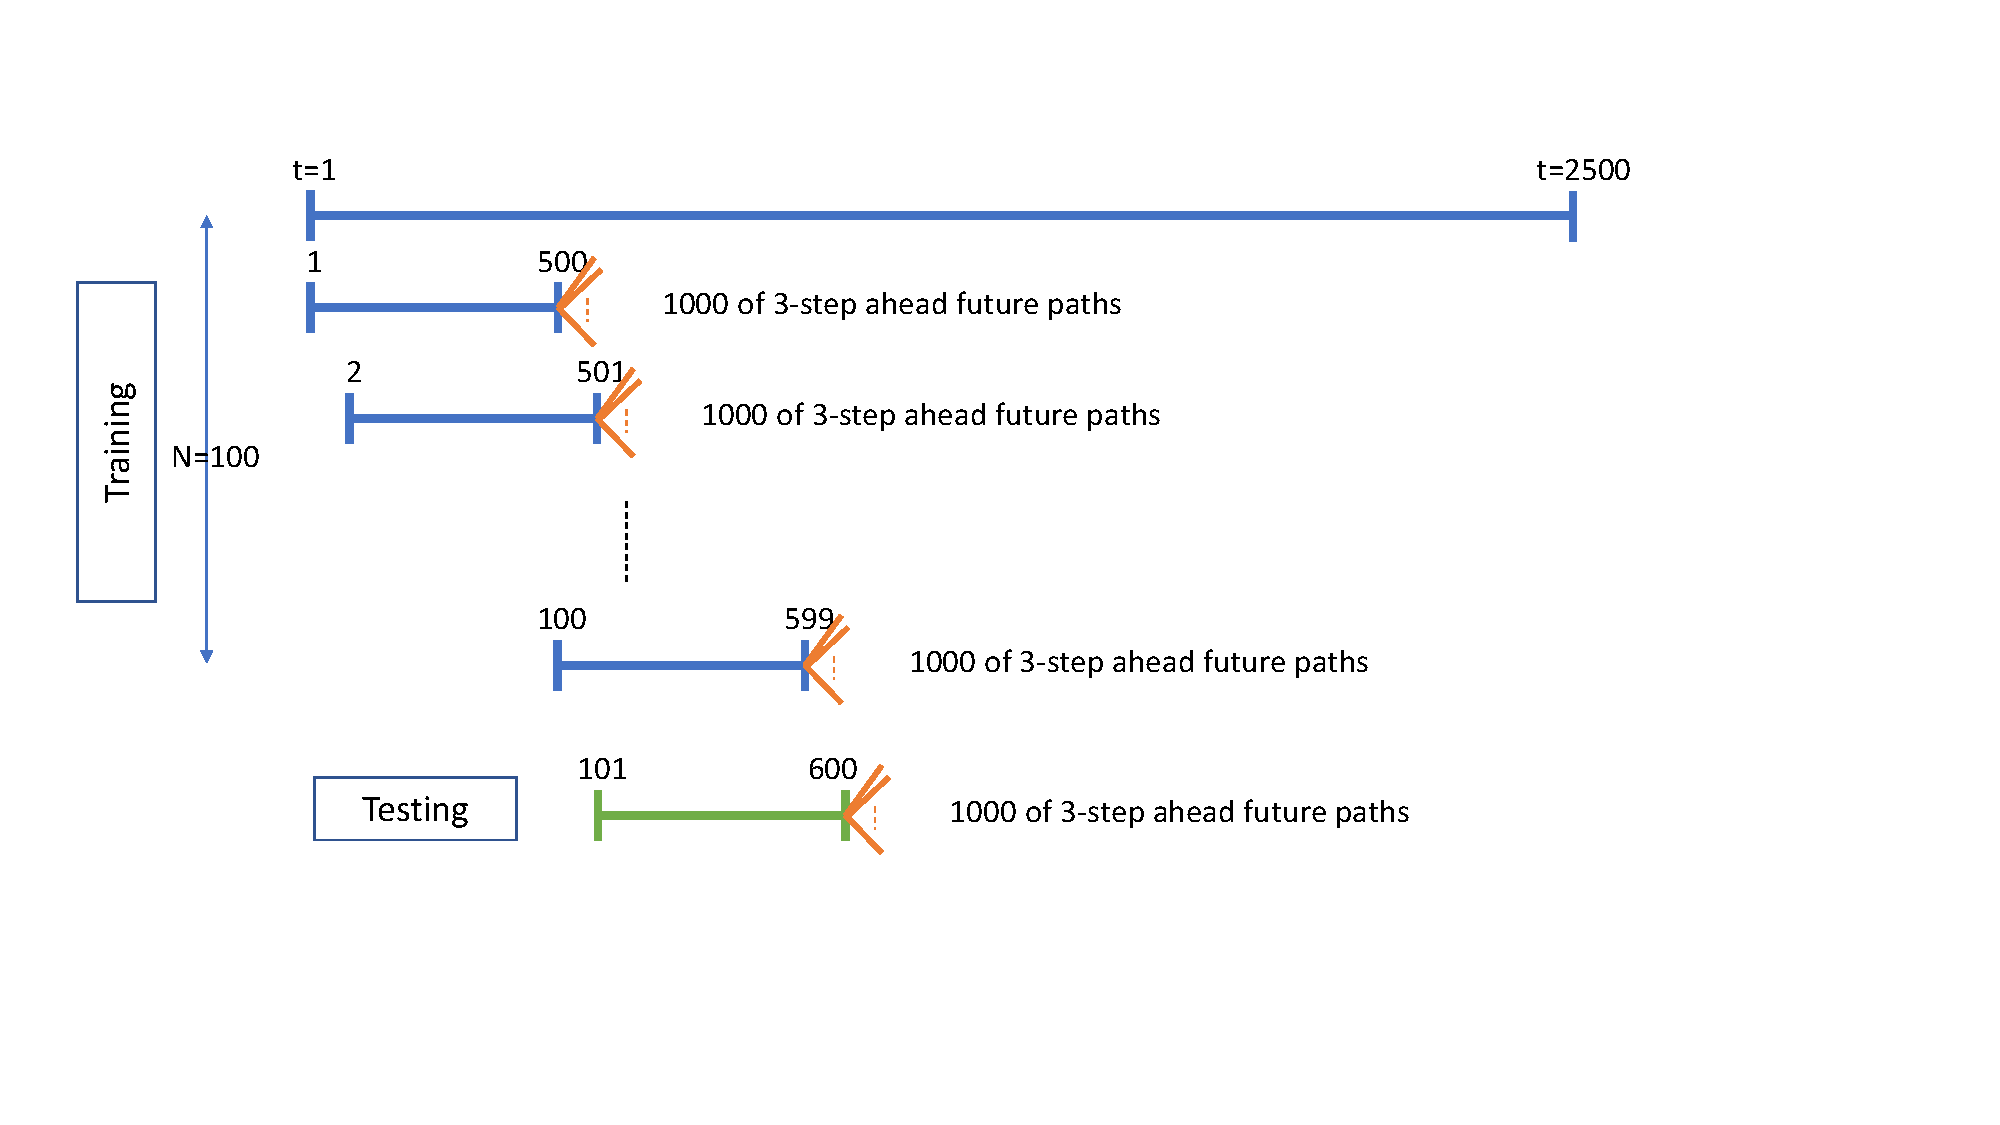
\includegraphics[scale=0.4]{Figs/Optimisation_TestingG.pdf}

\end{frame}

%------------------%

\begin{frame}{Monte-Carlo Simulation \textit{Cont.}}
\begin{itemize}
	\item Simulation setup: 
	\begin{itemize}[<+-| alert@+>]
		\item [$\bullet$] First 2500 observations were generated.
		\item [$\bullet$] Fit Univariate ARIMA models for a rolling window of 500 observations.
		\item [$\bullet$] $B=1000$ of $h=1,2,3$ steps-ahead bootstrap future paths generated.
		\item [$\bullet$] Training window is rolled one observation ahead and process was repeated until $N=100$ incoherent, $h=1,2,3$ steps-ahead future paths were generated.
		\item [$\bullet$] We find the optimal $\bm{G}_h$ for $h=1,2,3$ that reconciles $h$-step-ahead future paths giving minimal average Energy score. 
		\item [$\bullet$] This optimal $\bm{G}_h$ is then used to reconcile the incoherent future paths for the test set.
		\item [$\bullet$] The Process was repeated 1000 times and average scores were calculated for the test set.
	\end{itemize}
\end{itemize}
\end{frame}
%------------------%

\begin{frame}{Monte-Carlo Simulation \textit{Cont.}}
\begin{itemize}
	\item []
	\begin{table}
		
		\resizebox{\linewidth}{!}{
			\small
			\begin{tabular}{@{}lSSSSSSSS@{}}
				\toprule
				\multicolumn{1}{c}{Optimisation} &
				\multicolumn{4}{c}{\text{Hierarchy 1}} & 
				\multicolumn{4}{c}{\text{Hierarchy 2}} \\
				\cmidrule(lr){2-5} \cmidrule(lr){6-9} 
				\multicolumn{1}{c}{method} & \multicolumn{2}{c}{$h=1$} & \multicolumn{2}{c}{$h=3$} & \multicolumn{2}{c}{$h=1$} & \multicolumn{2}{c}{$h=3$} \\
				\cmidrule(lr){2-3} \cmidrule(lr){4-5} \cmidrule(lr){6-7} \cmidrule(lr){8-9} 
				& \text{ES} & \text{VS} & \text{ES} & \text{VS} & \text{ES} & \text{VS} & \text{ES} & \text{VS} \\   
				
				\midrule
				Method 1 - Optimising $\bm{W}$   			& 2.48 & 0.11 & 2.75 & 0.11 & 5.36 & 1.21 & 5.83 & 1.38  \\
				Method 2 - Optimising $\bm{R}$    			& 2.48 & 0.11 & 2.75 & 0.11 & 5.37 & 1.21 & 5.83 & 1.37  \\
				Method 3 - Optimising $\bm{R}$(Restricted)  & 2.48 & 0.11 & 2.75 & 0.11 & 5.37 & 1.21 & 5.83 & 1.37  \\
				Method 4 - Optimising $\bm{G}$   			& 2.48 & 0.11 & 2.75 & 0.11 & 5.38 & 1.21 & 5.83 & 1.38  \\
				\bottomrule
				
			\end{tabular}
		}
	\end{table}
	\item[]
	\item Parameterisation does not matter
\end{itemize}
\end{frame}

%------------------%

\begin{frame}{Monte-Carlo Simulation \textit{Cont.}}
\begin{itemize}
	\item Comparison with point forecast reconciliation methods.
	\item[]
	\begin{table}
		\resizebox{\linewidth}{!}{
			\small
			\begin{tabular}{@{}lSSSSSSSS@{}}
				\toprule
				\multicolumn{1}{c}{Reconciliation} &
				\multicolumn{4}{c}{\text{Hierarchy 1}} & 
				\multicolumn{4}{c}{\text{Hierarchy 2}} \\
				\cmidrule(lr){2-5} \cmidrule(lr){6-9} 
				\multicolumn{1}{c}{method} & \multicolumn{2}{c}{$h=1$} & \multicolumn{2}{c}{$h=3$} & \multicolumn{2}{c}{$h=1$} & \multicolumn{2}{c}{$h=3$} \\
				\cmidrule(lr){2-3} \cmidrule(lr){4-5} \cmidrule(lr){6-7} \cmidrule(lr){8-9} 
				& \text{ES} & \text{VS} & \text{ES} & \text{VS} & \text{ES} & \text{VS} & \text{ES} & \text{VS} \\   
				
				\midrule
				Optimal $\bm{G}$   	& 2.48* & 0.106 & 2.75* & 0.106 & 5.36* & 1.21* & 5.83* & 1.38*\\
				MinT(Shrink)    	& 2.47* & 0.105 & 2.74* & 0.105 & 5.33* & 1.19* & 5.77* & 1.34*\\			
				WLS   				& 2.46* & 0.105 & 2.74* & 0.105 & 5.43* & 1.23 & 5.98* & 1.40* \\
				OLS 				& 2.54* & 0.105 & 2.80* & 0.105 & 5.51* & 1.23 & 5.98* & 1.40*\\
				\textit{Base} 		& $\textit{2.67}$ & $\textit{0.105}$ & $\textit{2.94}$ & $\textit{0.105}$ & $\textit{5.71}$ & $\textit{1.28}$ & $\textit{6.27}$ & $\textit{1.49}$\\   			
				\bottomrule
				 \multicolumn{9}{l}{\text{``*'' indicates if the average score for a particular reconciliation method is significantly }}\\
				 \multicolumn{9}{l}{\text{different from that of base forecasts.}}
				 
			\end{tabular}
		}
	\end{table}
	\item[]
	\item Reconciliation methods perform better than Base forecasts.
	\item[]
	\item MinT(Shrink) is at least as good as Optimal method. Thus going forward with MinT projection. 
	
\end{itemize}
\end{frame}

%------------------%



%%-------------------------------


%%-------------------------------
%-------------------------


%----------------------

\section{Project 3: Hierarchical forecasts for macroeconomic variables - An application to Australian GDP}

\begin{frame}
\frametitle[]
%\frametitle{A first slide}

\begin{center}
	\Huge Project 3: Hierarchical forecasts for macroeconomic variables - An application to Australian GDP
\end{center}
\end{frame}

%------------------%

\begin{frame}[noframenumbering]{Macroeconomic forecasting}
\begin{itemize}[<+-| alert@+>]
	\item[] 
	\begin{figure}
		\begin{overprint}
			\resizebox{\linewidth}{!}
{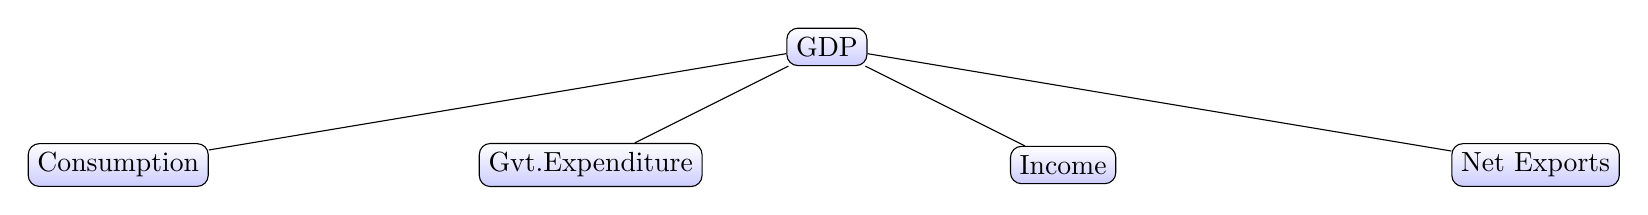
\begin{tikzpicture}[level/.style={sibling distance = 6cm/#1},
every node/.style = {shape=rectangle, rounded corners,
	draw, align=center,
	top color=white, bottom color=blue!20}]
\node {GDP}
child {node{Consumption}}
child {node{Gvt.Expenditure}}
child {node{Income}}
child {node{Net Exports}};
\end{tikzpicture}}
		\end{overprint}
	\end{figure}
	\item Common forecasting approaches involves univariate methods or multivariate methods such as VAR.
	\item[]
	\item The era of big data led to the use of regularization and shrinkage methods - dynamic factor models, Lasso, Bayesian VARs.
	\item[]
	\item The predictors in these methods commonly include the components of the variables of interest. 
	\item[]
	\item This might fail to reflect the deterministic relationship between macroeconomic variables in the forecasts.
	\end{itemize}
\end{frame}

\begin{frame}{Macroeconomic forecasting}
\begin{itemize}[<+-| alert@+>]
	\item Both aligned decision making and forecast accuracy are key concerns for economic agents and policy makers.
	\item[]
	\item Thus we propose to use hierarchical forecasting methods in macroeconomic forecasts.
	\item[]
	\item Related literature: Only one application on point forecasting for inflation \citep{capistran2010multi,weiss2018essays}
	\item[]
	\item To the best of our knowledge we use hierarchical forecasting methods for point as well as probabilistic forecasts for the first time in macroeconomic literature. 
\end{itemize}
\end{frame}


%------------------%

\begin{frame}{Australian GDP : \textit{Data structures}}
\begin{itemize}[<+-| alert@+>]
	\item We consider Gross Domestic Product (GDP) of Australia with quarterly data spanning the period 1984:Q4--2018:Q3.
	\item[]
	\item The Australian Bureau of Statistics (ABS) measures GDP using three main approaches - Production, Income and Expenditure.
	\item[] The final GDP figure is obtained as an average of these three figures.
	\item[]
	\item We restrict our attention to nominal, seasonally unadjusted data.
	\item[]
	\item Thus we concentrate on the Income and Expenditure approaches.  
\end{itemize}
\end{frame}


%------------------%

\begin{frame}{Australian GDP : \textit{Data structures}}
\begin{itemize}[<+-| alert@+>]
	\item[] 
	
\begin{block}{Income approach}
		\begin{align*}
	\textit{GDP}
	& = \textit{Gross operating surplus} + \textit{Gross mixed income} \\
	& + \textit{Compensation of employees} \\
	& + \textit{Taxes less subsidies on production and imports} \\
	& + \textit{Statistical discrepancy (I)}.
	\end{align*}
\end{block}
	\item  The hierarchy has two levels of aggregation below the top-level, with a total of $n=16$ series and $m=10$ bottom level series.

\end{itemize}
\end{frame}


%------------------%

\begin{frame}{Australian GDP : \textit{Data structures - Income approach}}
\begin{itemize}[<+-| alert@+>]
	\item[] 
	\begin{figure}
		\resizebox{\linewidth}{!}{
		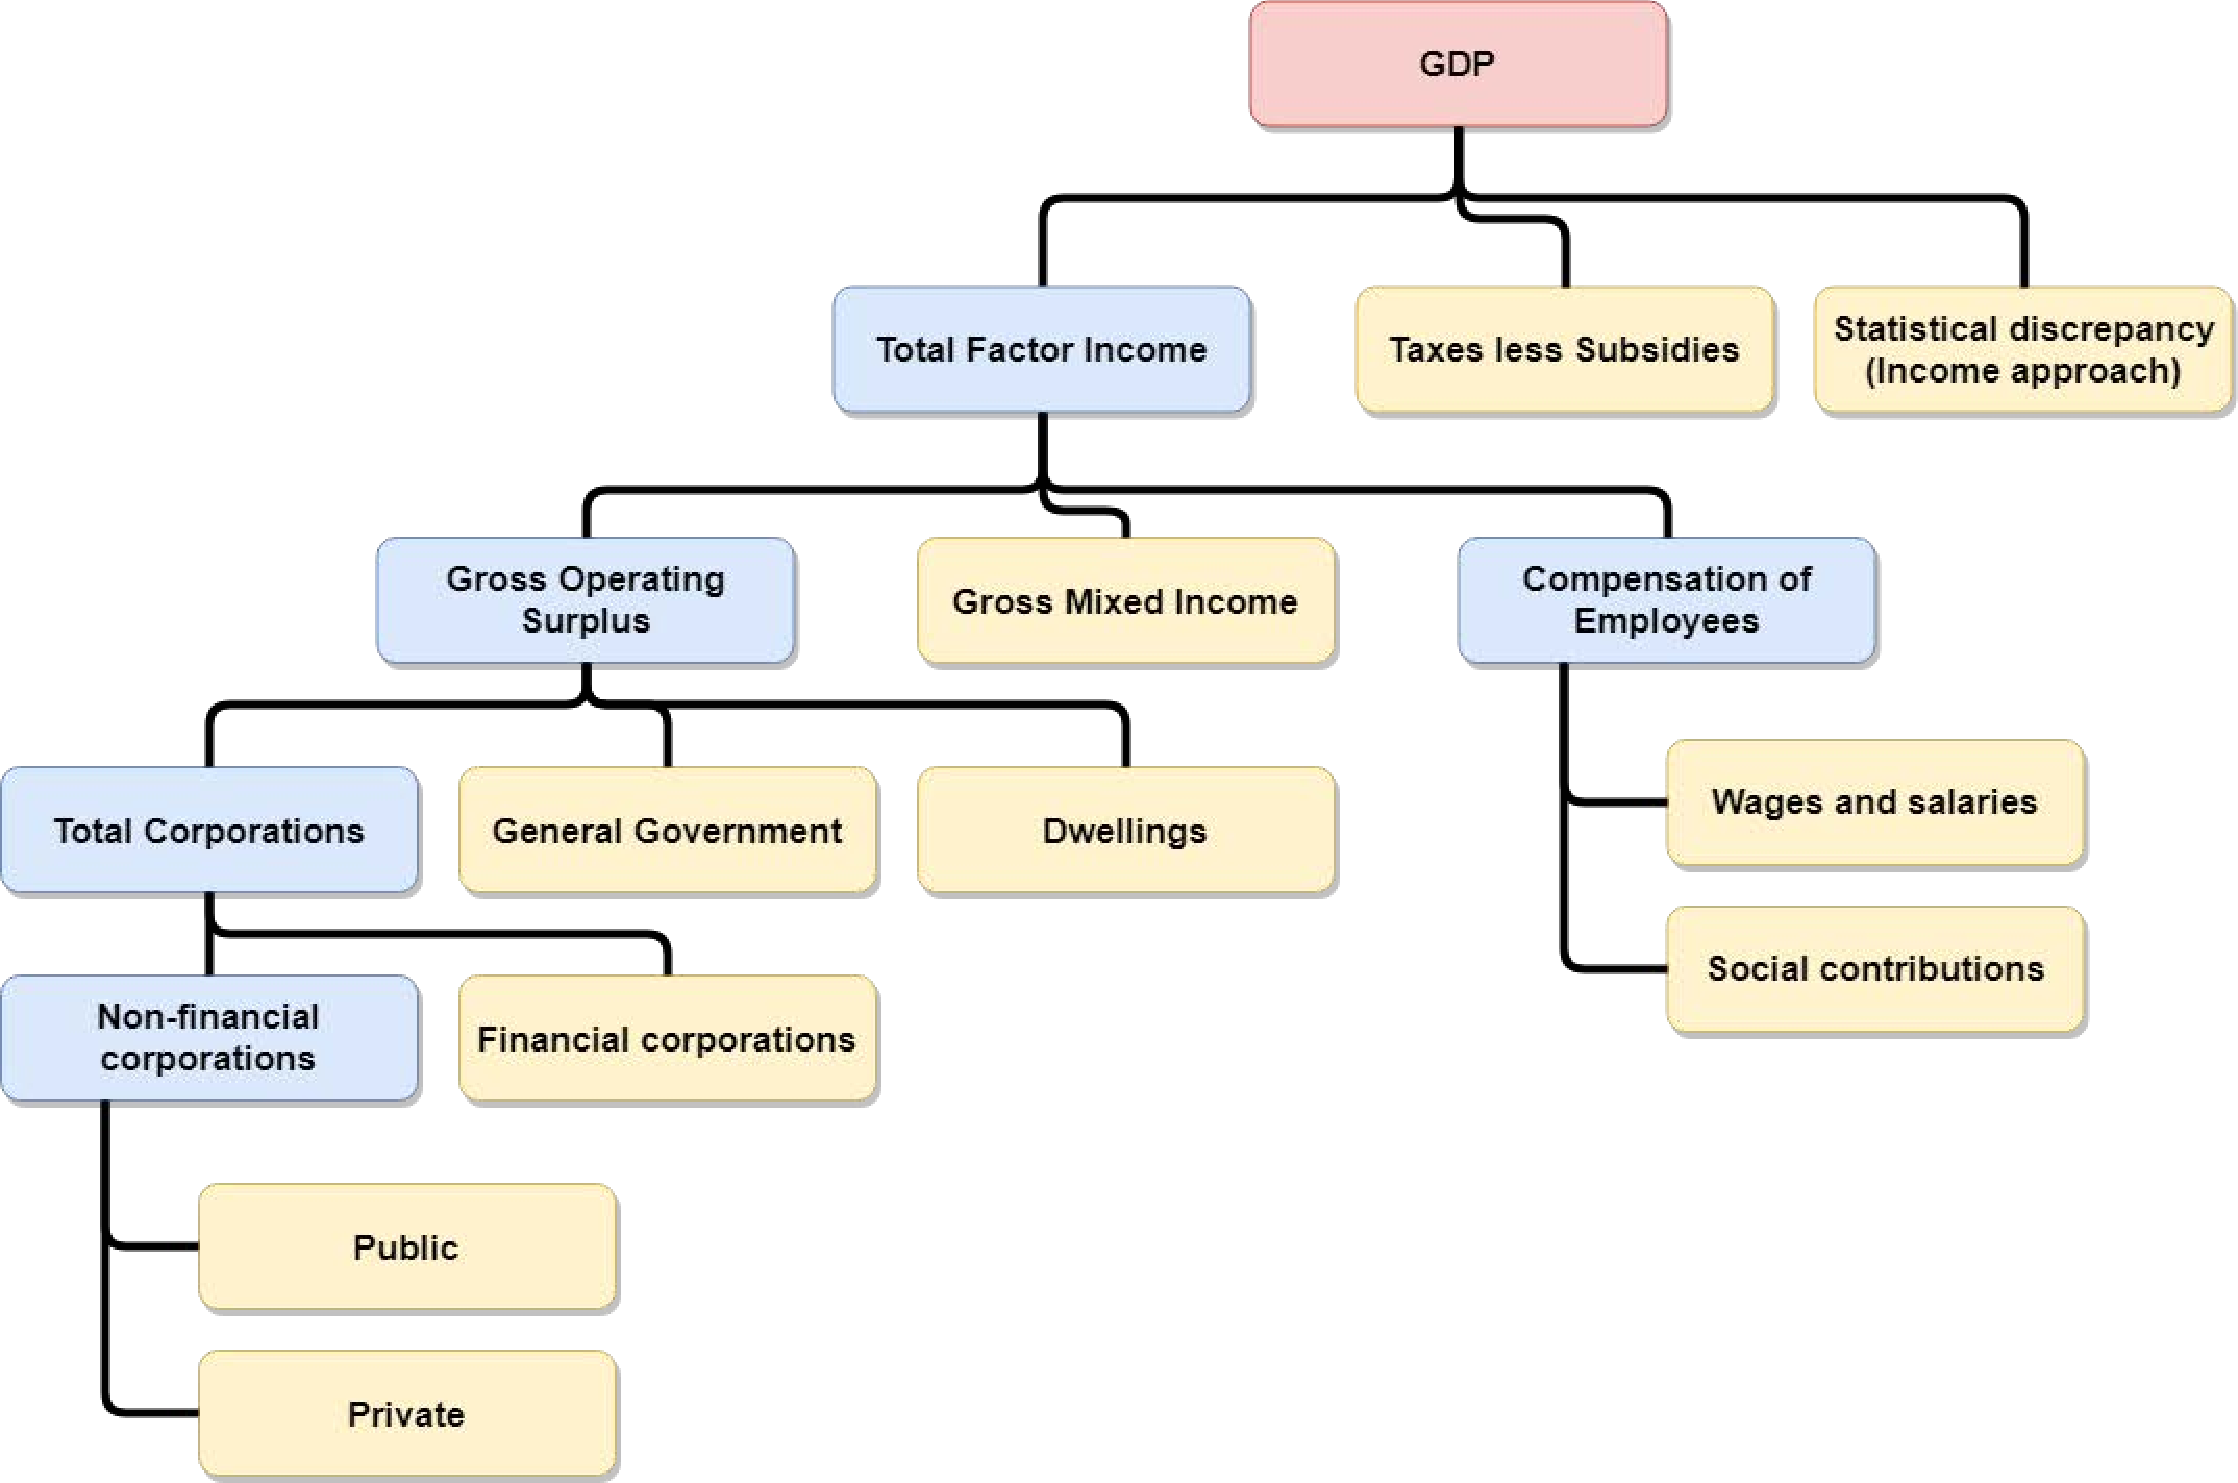
\includegraphics[]{Figs/Hierarchical-structures/IncomeApproach}
	}
	\end{figure}	
	
\end{itemize}
\end{frame}


%------------------%

\begin{frame}{Australian GDP : \textit{Data structures}}
\begin{itemize}[<+-| alert@+>]
	\item[] 
	
	\begin{block}{Expenditure approach}
		\begin{align*}
		\textit{GDP}
		& = \textit{Final consumption expenditure}
		+ \textit{Gross fixed capital formation} \\
		& + \textit{Changes in inventories}
		+ \textit{Trade balance}\\
		&+ \textit{Statistical discrepancy (E)}.
		\end{align*}
	\end{block}
	
	\item The hierarchy has three levels of aggregation below the top-level, with a total of $n=80$ series and $m=53$ series at the bottom level.
	
\end{itemize}
\end{frame}


%------------------%

\begin{frame}{Australian GDP : \textit{Data structures - Expenditure approach}}
\begin{itemize}[<+-| alert@+>]
\item[] 
\begin{figure}
	\vspace{-0.7cm}
	\resizebox{\linewidth}{!}{
		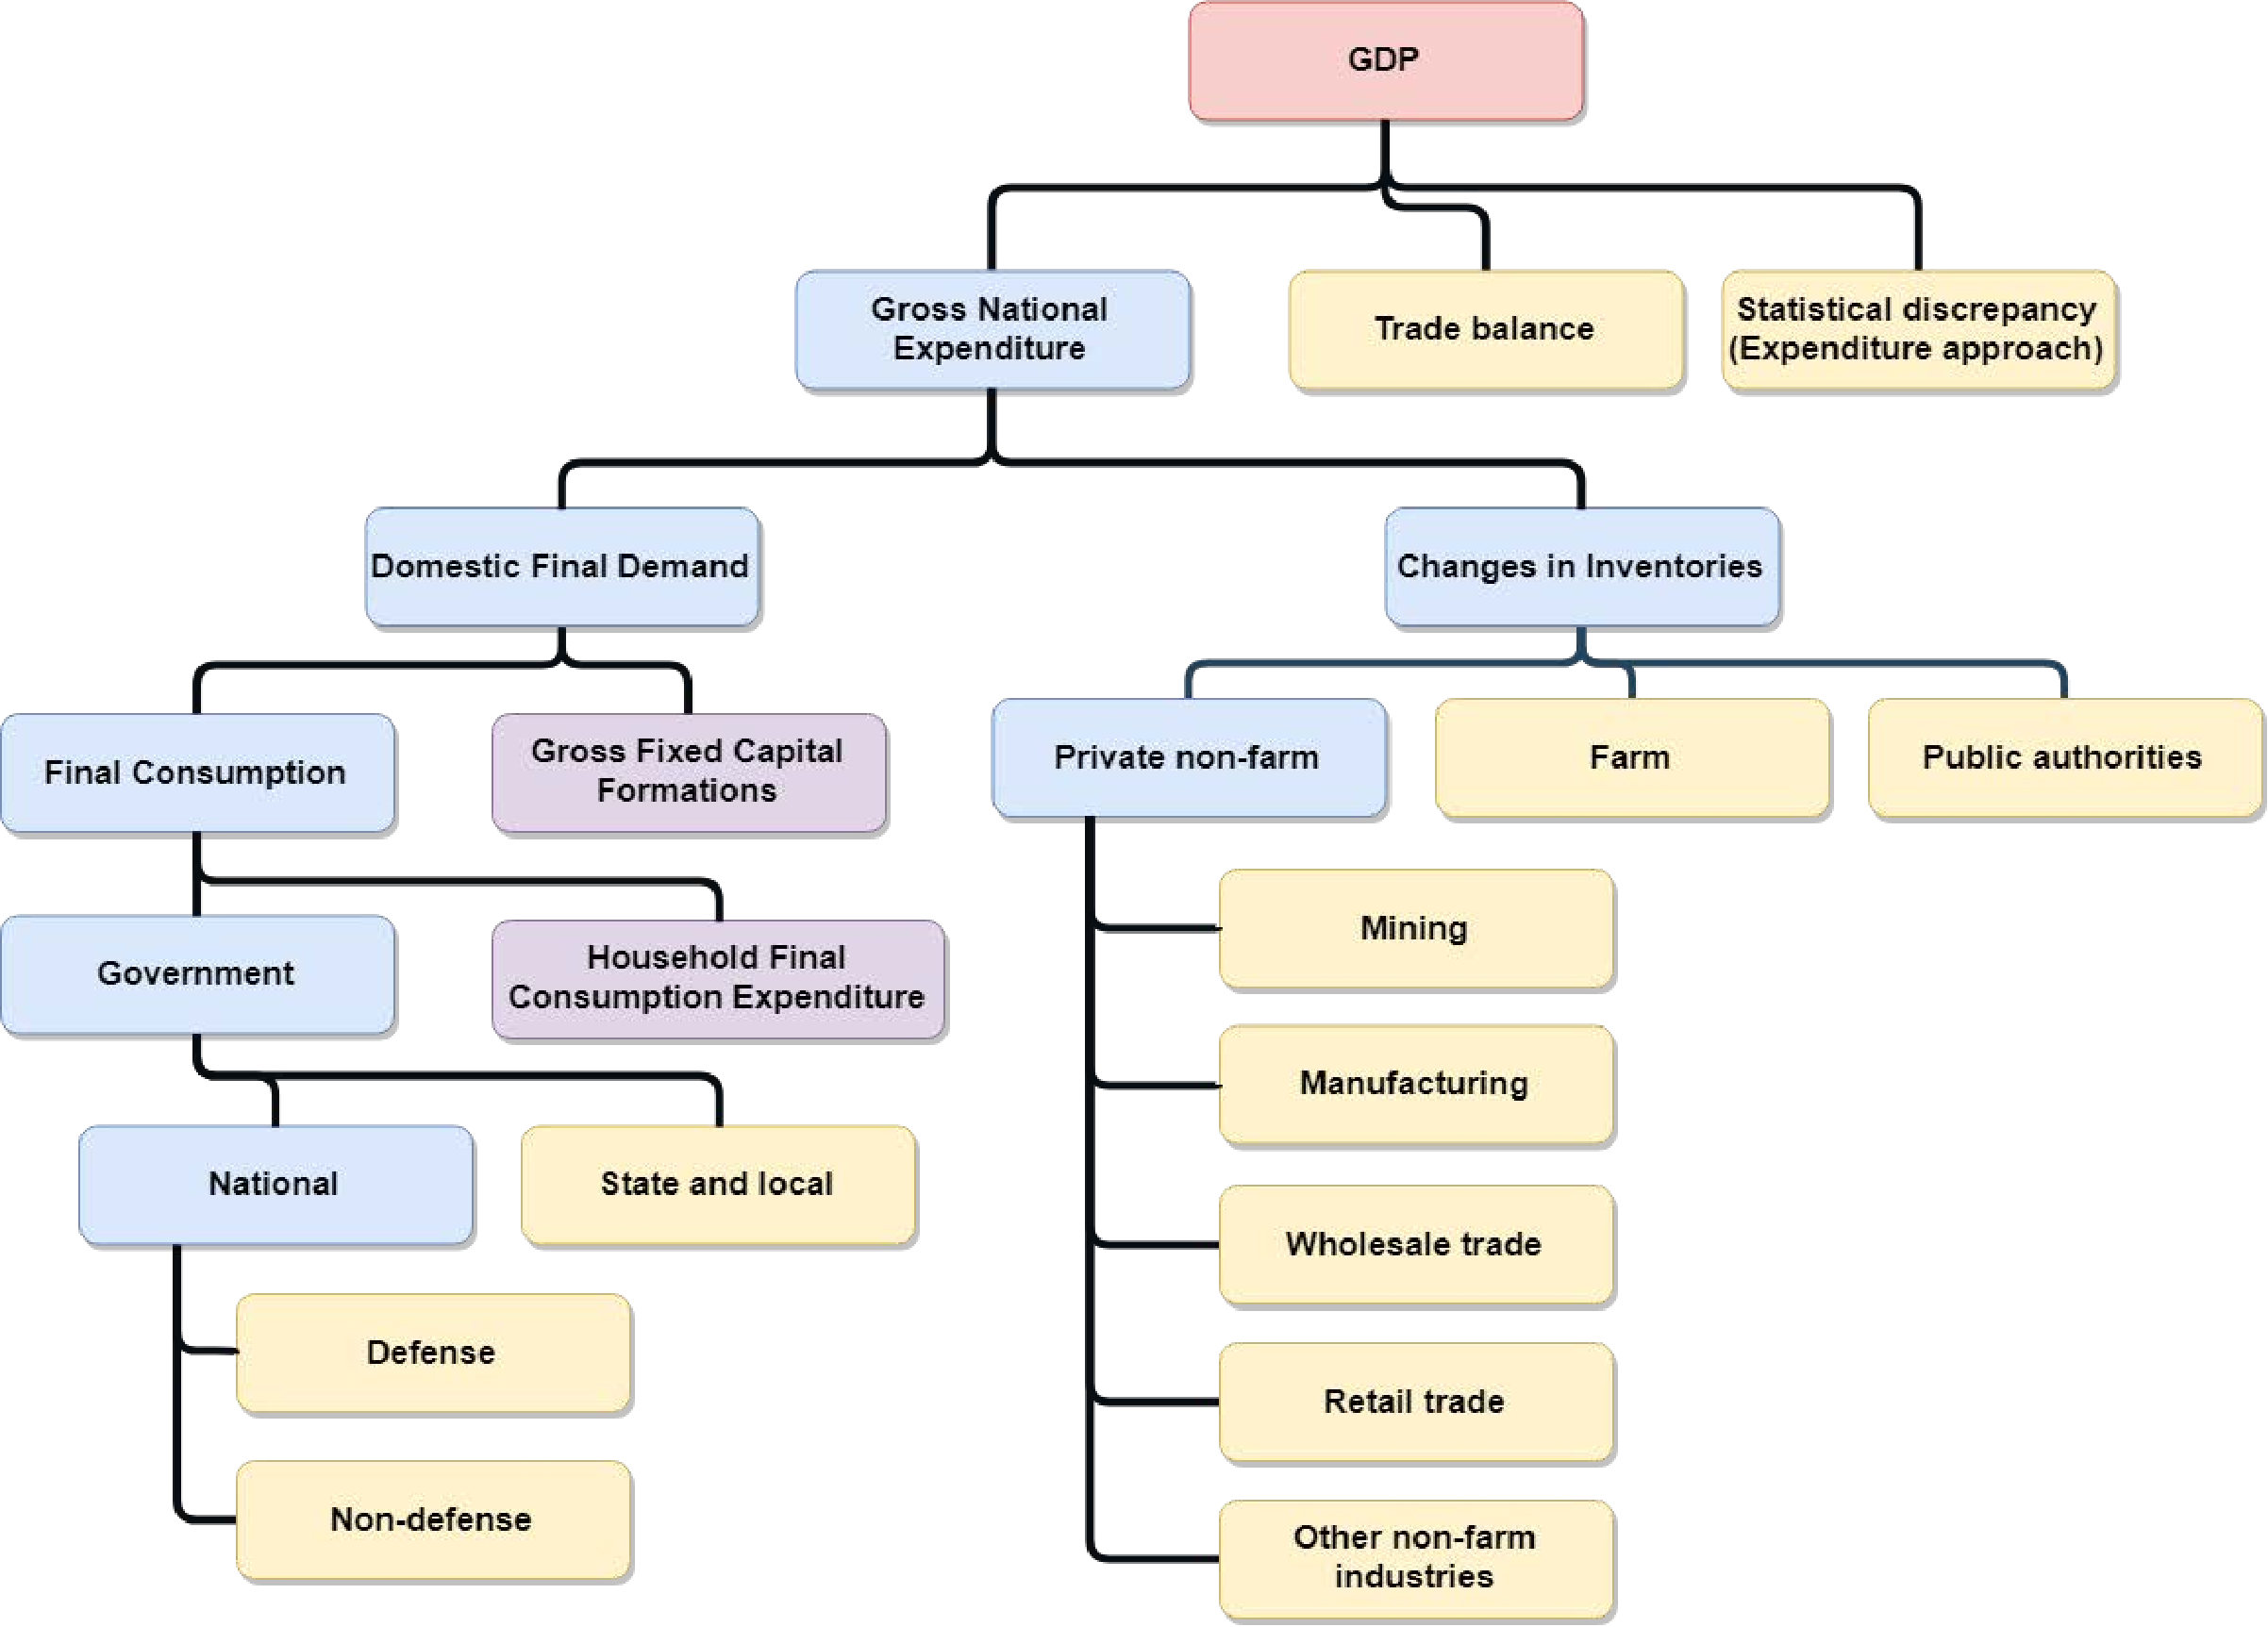
\includegraphics[width=.9\textwidth]{Figs/Hierarchical-structures/ExpenditureApproach.pdf}
	}
\end{figure}	

\end{itemize}
\end{frame}


%------------------%

\begin{frame}{Australian GDP : \textit{Data structures - Expenditure approach}}
\begin{itemize}[<+-| alert@+>]
	\item[] 
	\begin{figure}
		\vspace{-0.7cm}
		\centering
		\resizebox{\linewidth}{!}{
			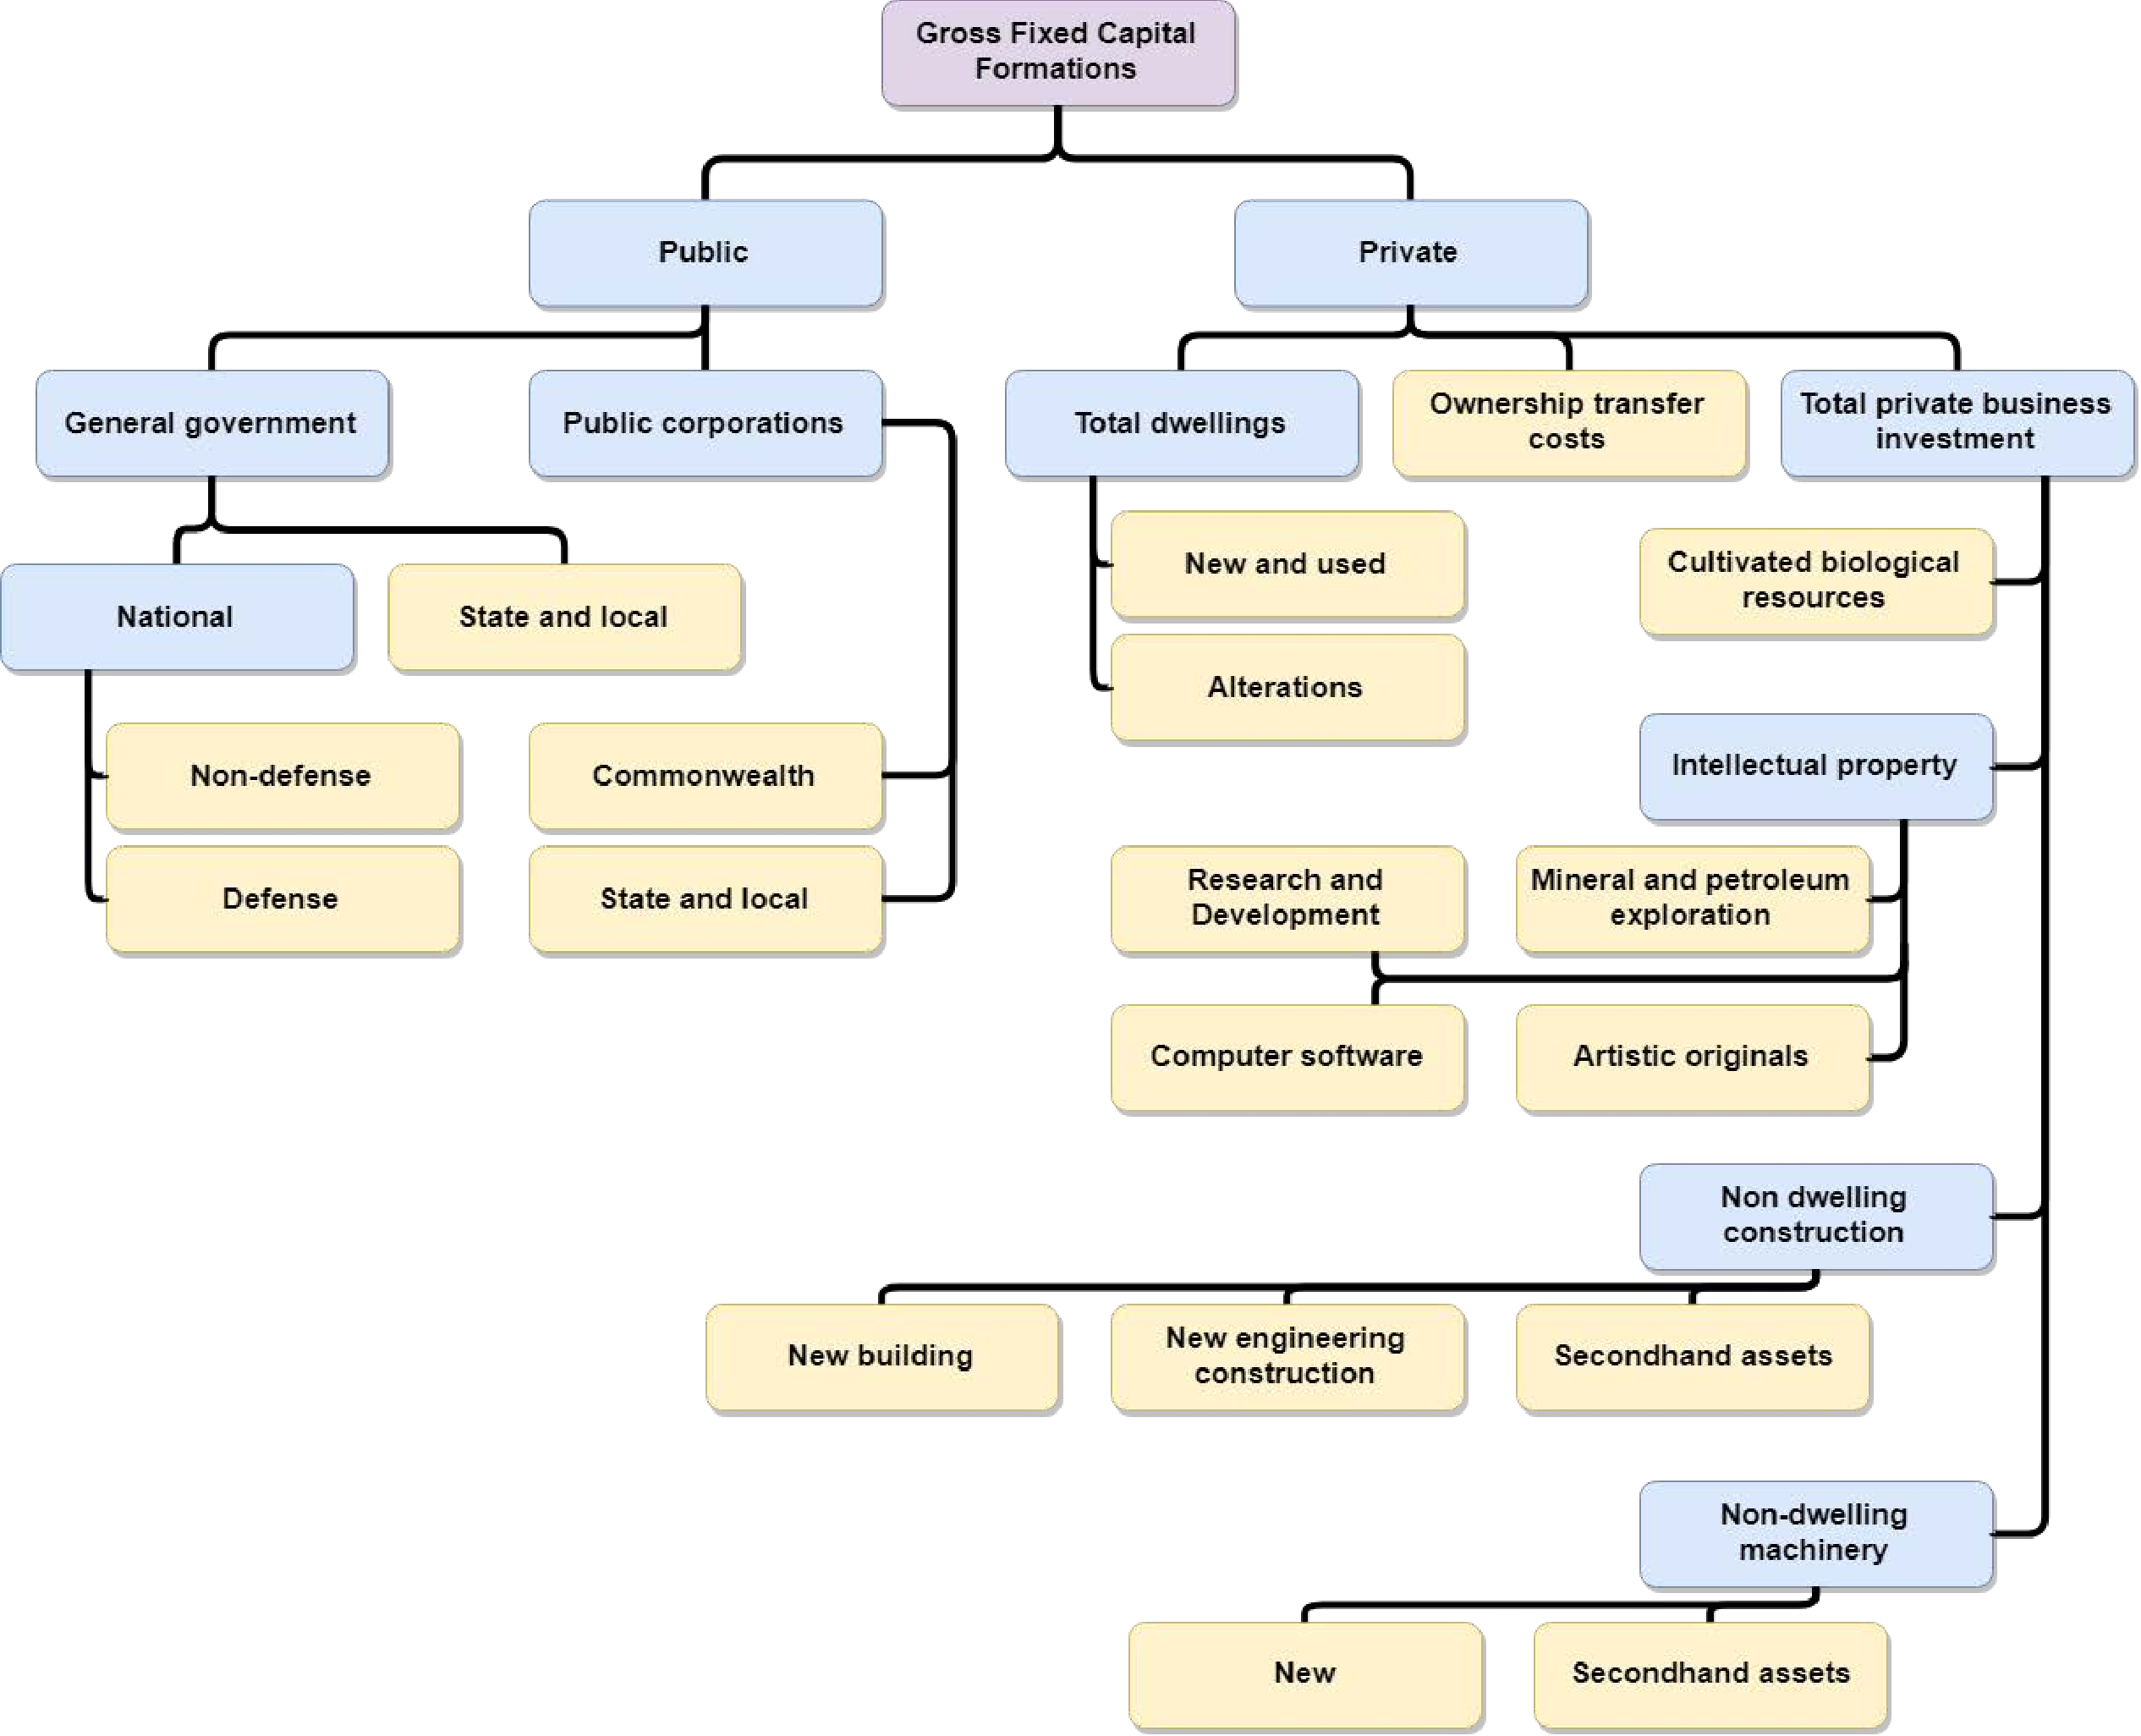
\includegraphics[scale=0.03]{Figs/Hierarchical-structures/GFCF.pdf}
		}
	\end{figure}	
	
\end{itemize}
\end{frame}


%------------------%

\begin{frame}{Australian GDP : \textit{Data structures - Expenditure approach}}
\begin{itemize}[<+-| alert@+>]
	\item[] 
	\begin{figure}
		\vspace{-0.7cm}
		\centering
		\resizebox{\linewidth}{!}{
			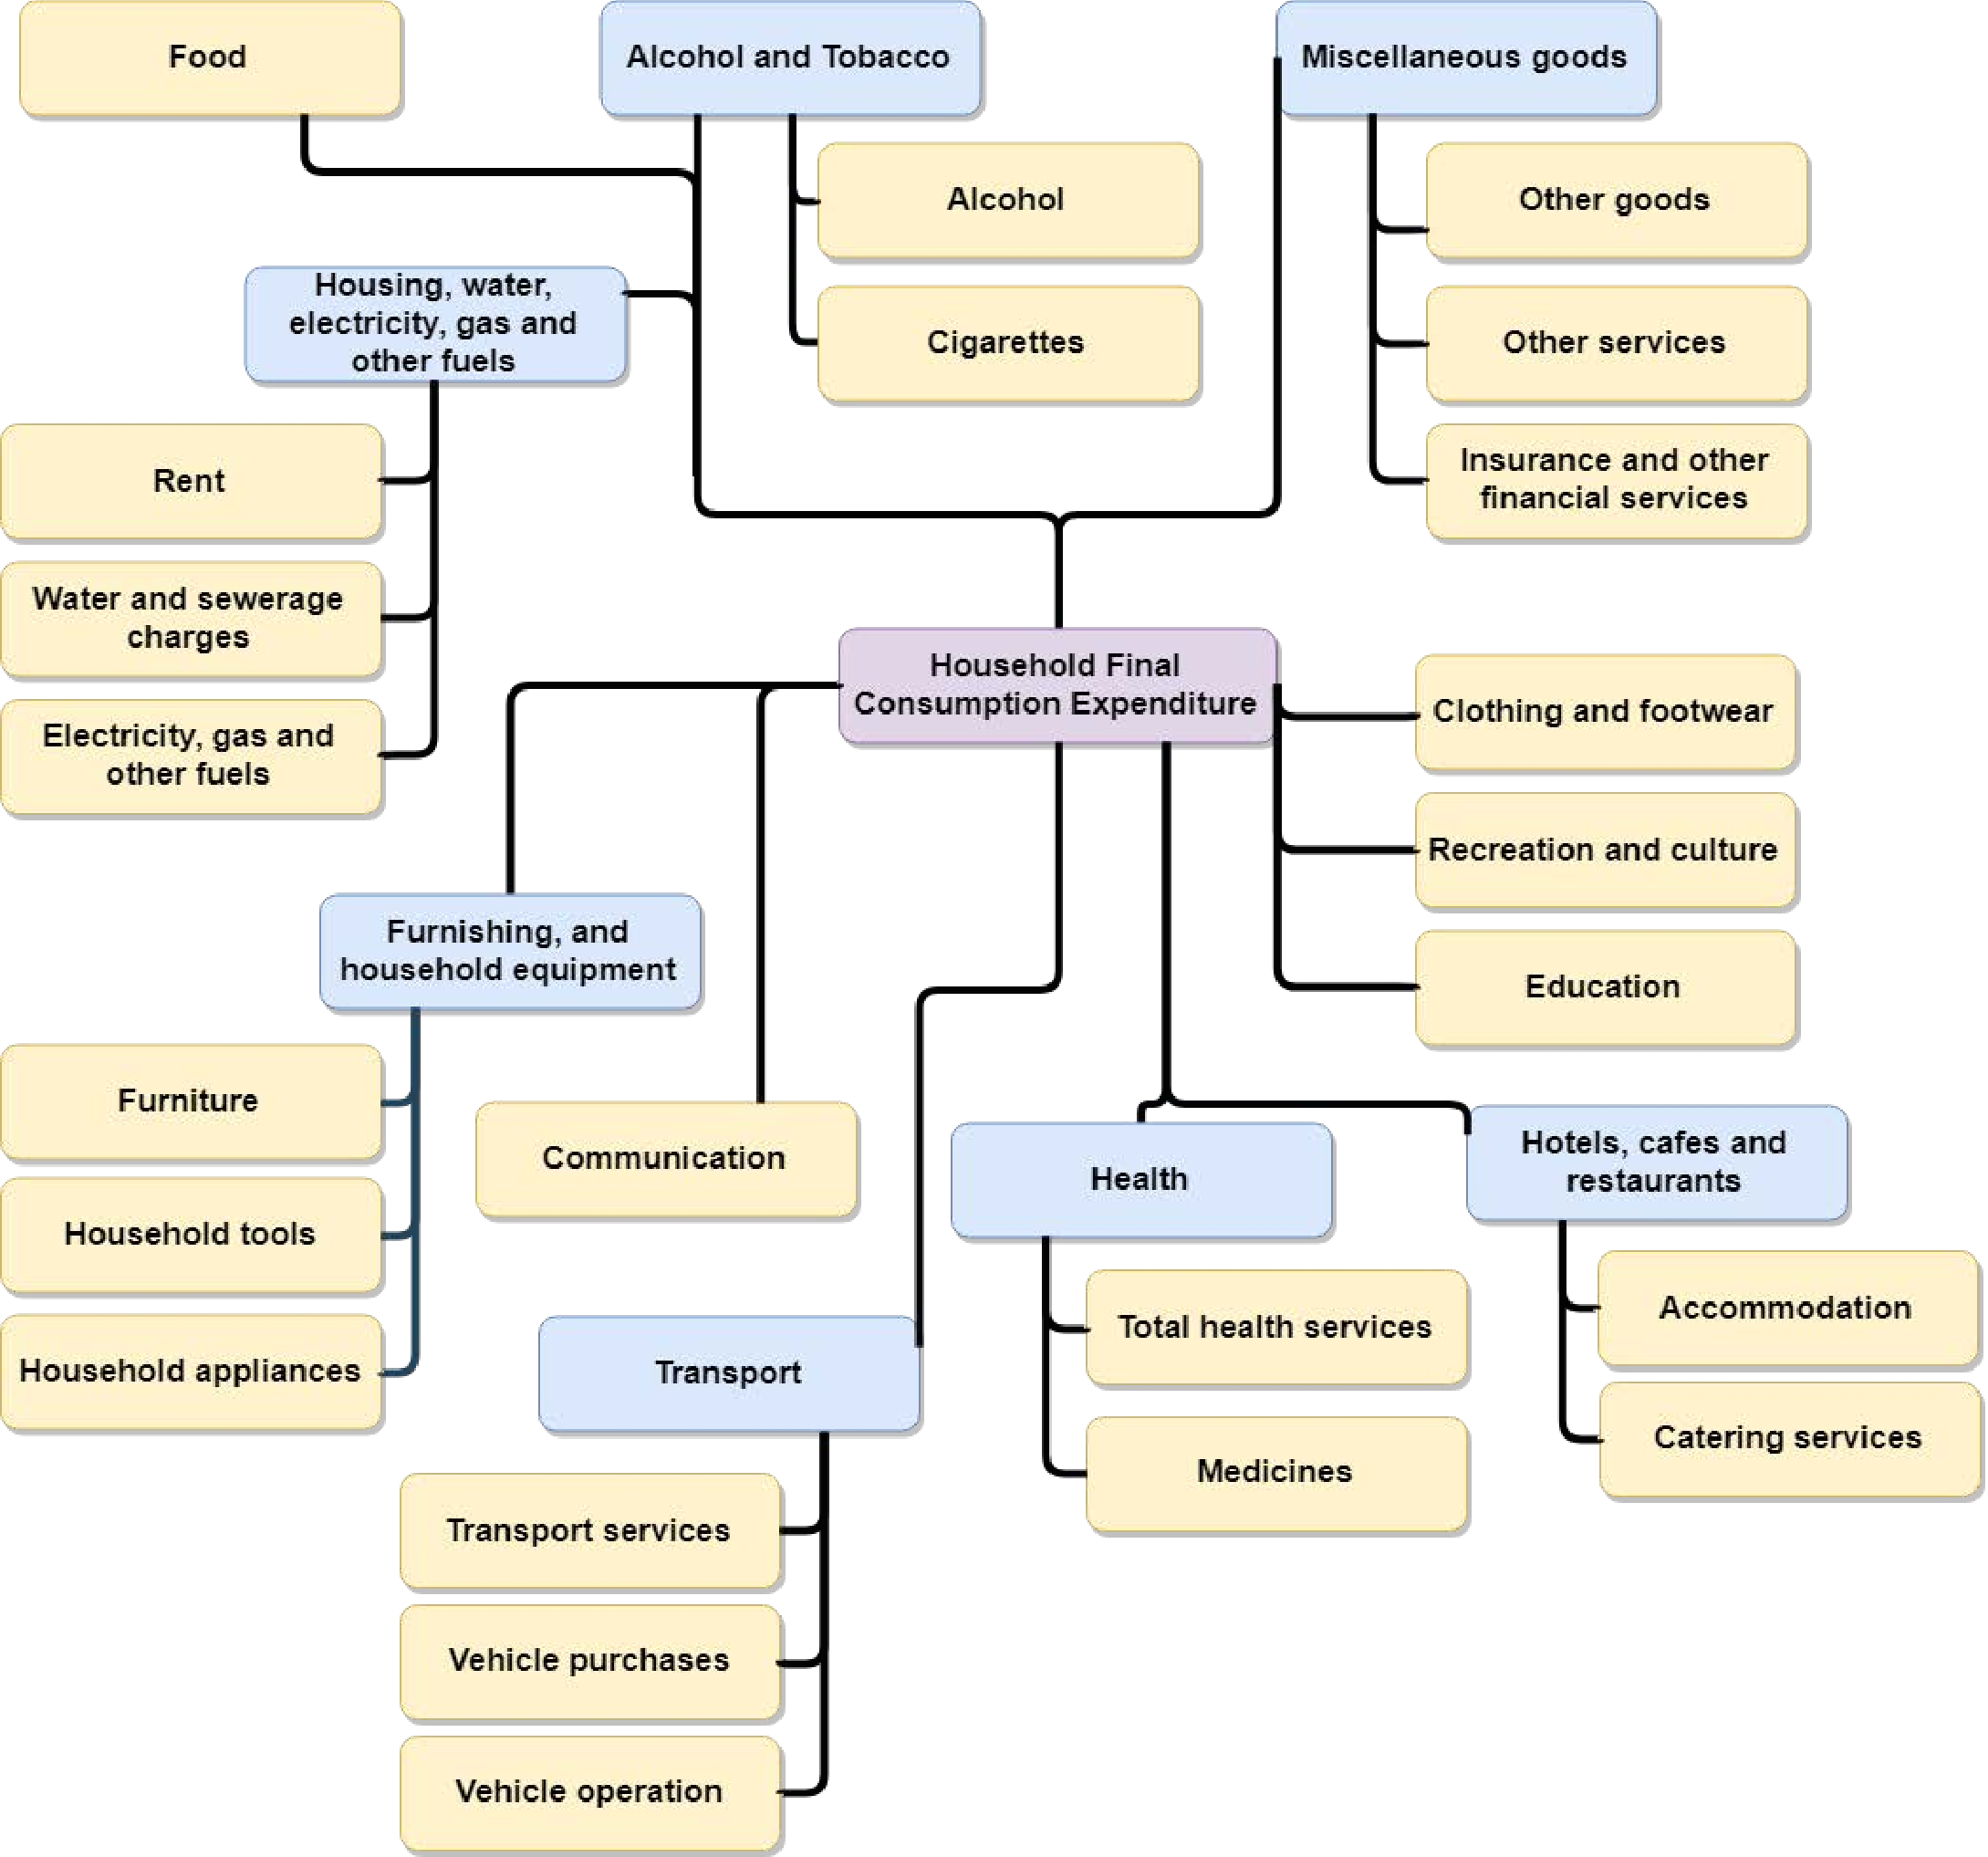
\includegraphics[scale=0.01]{Figs/Hierarchical-structures/HFCE.pdf}
		}
	\end{figure}	
	
\end{itemize}
\end{frame}


%------------------%

\begin{frame}{Australian GDP : \textit{Time plots for different levels}}
\begin{itemize}[<+-| alert@+>]
	\item[] 
	\begin{figure}

		\centering
		\small
		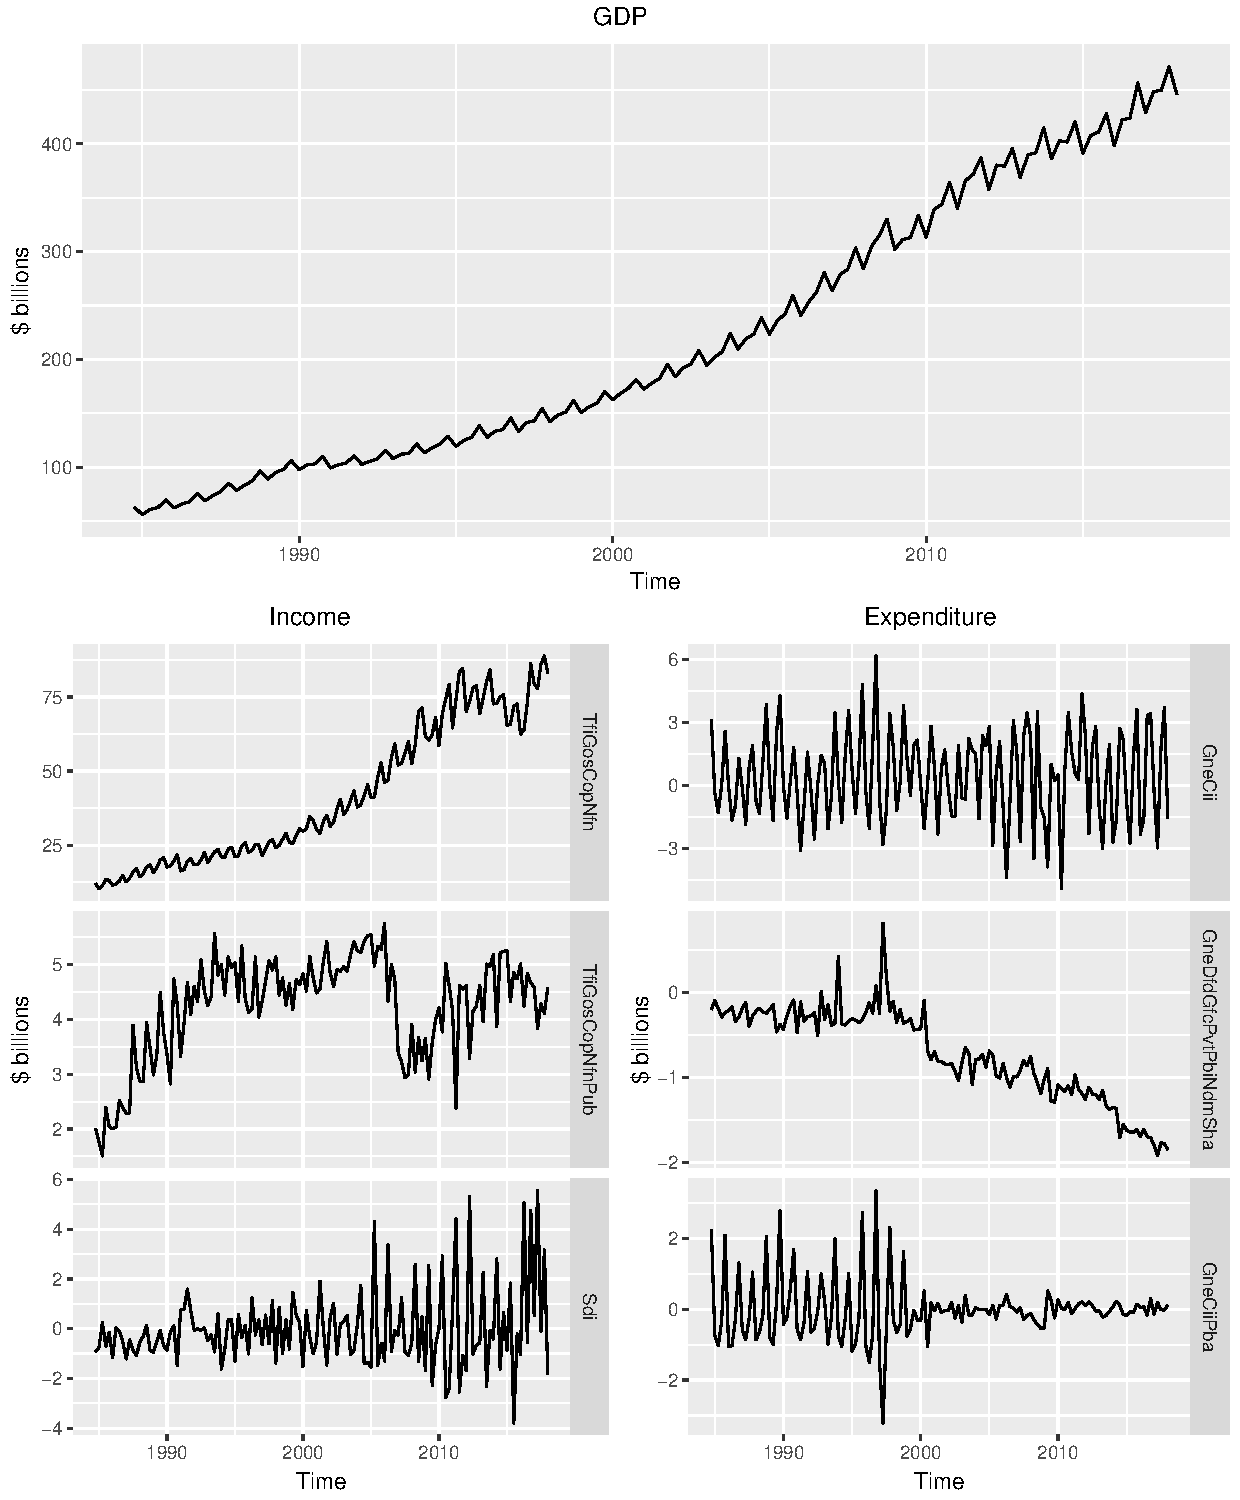
\includegraphics[scale=0.30]{Figs/TS-plots/TSplots-INC-EXP.pdf}
		
	\end{figure}
	
\end{itemize}
\end{frame}


%------------------%

\begin{frame}{Methodology}
\begin{itemize}[<+-| alert@+>]
	\item \textbf{Analysis set up:}
	\begin{itemize}[<+-| alert@+>]
		\item[$\bullet$] First training sample is set from 1984:Q4 to 1994:Q3 and forecasts produces for four quarters ahead (1994:Q4 to 1995:Q3).
		\item[$\bullet$] Then the training window is expanded by one quarter at a time.
		\item[$\bullet$] This leads to 94 1-step-ahead, 93 2-steps-ahead, 92 3-steps-ahead and 91 4-steps-ahead forecasts available for evaluation. 
	\end{itemize}
	\item[]
	\item \textbf{Base forecasting models:}
	\begin{itemize}[<+-| alert@+>]
		\item[$\bullet$] Univariate ARIMA and ETS models were fitted for each training set. \item[$\bullet$] $h=1,2,3,4$ steps ahead forecasts were generated using the fitted models.
	\end{itemize}
	
\end{itemize}
\end{frame}


%------------------%
\begin{frame}{Point forecasts: \textit{Base vs Seasonal \Naive}}
\begin{itemize}[<+-| alert@+>]
	\item[] 
	\resizebox{\linewidth}{!}{
	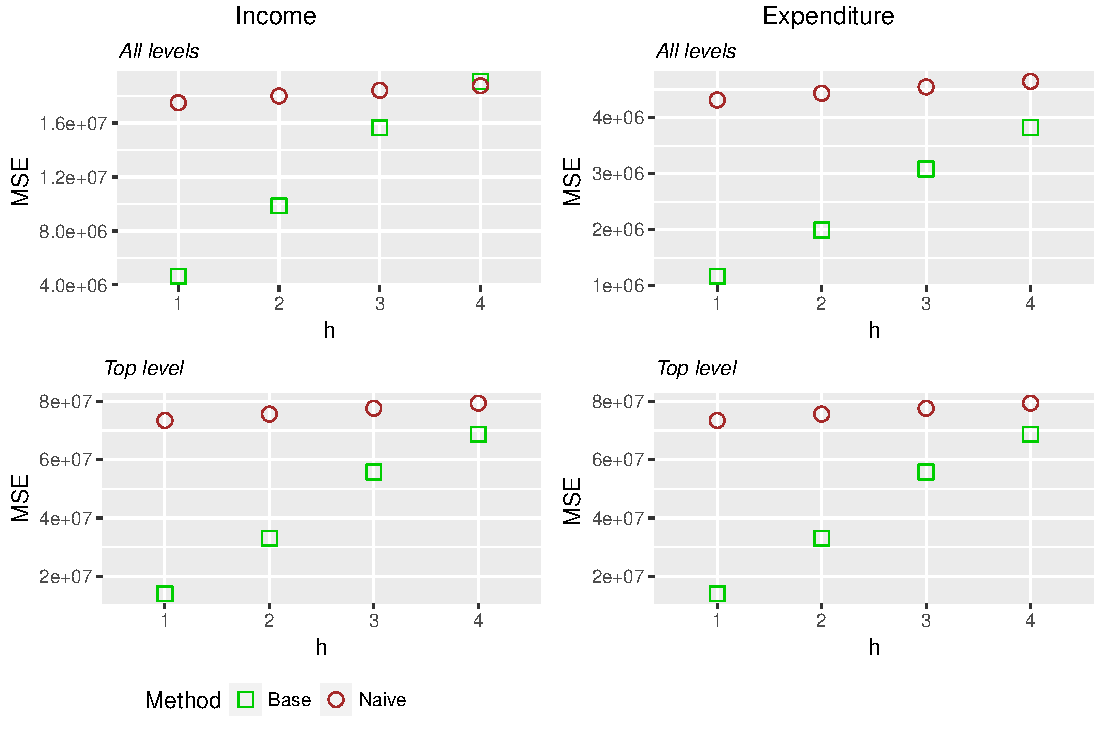
\includegraphics[width=\textwidth,height=\textheight,keepaspectratio]{Figs/Results/NaiveVsBase_MSE.pdf}
	}
	
	
\end{itemize}
\end{frame}


%------------------%



\begin{frame}{Point forecasts: \textit{Reconciliation}}
\begin{itemize}[<+-| alert@+>]
	\item[] Reconciled forecasts are given by,
	\begin{equation*}
	\color{Maroon}\tilde{\bm y}_{T+h} = \bm{SG}\hat{\bm y}_{T+h}
	\end{equation*}
		\item[]
	\begin{center}
		\begin{block}{}
			\begin{table}
				\small
				\centering %\setstretch{1.5}
				\begin{tabular}{lc}
					\toprule
					\textbf{Method} & \textbf{$\bm{G}$} \\
					\midrule
					BU             & $\left(\bm{0}_{m\times n-m}~\bm{I}_{m\times m}\right)$\\
					OLS             &
					$\left(\bm{S}'\bm{S}\right)^{-1}{\bm S'}$  \\
					WLS    &
					$\left(\bm{S}'\bm{\hat{W}}_{T+1}^{wls}\bm{S}\right)^{-1}\bm{S}'\bm{\hat{W}}_{T+1}^{wls}$ \\
					MinT(Shrink)    &
					$\left(\bm{S}'\bm{\hat{W}}_{T+1}^{shr}\bm{S}\right)^{-1}\bm{S}'\bm{\hat{W}}_{T+1}^{shr}$ \\
					\bottomrule
				\end{tabular}
			\end{table}
		\end{block}
	\begin{table}
		\small
		\centering %\setstretch{1.5}
		\begin{tabular}{lll}
			\toprule
			$\bm{\hat{W}}_{T+1}^{shr}$ & = & $\tau\text{Diag}(\bm{\hat{W}}_{T+1}^{sam}) + (1-\tau)\bm{\hat{W}}_{T+1}^{sam}$\\
			$\bm{\hat{W}}_{T+1}^{wls}$ & = & $\text{Diag}(\bm{\hat{W}}_{T+1}^{shr})$\\
			\bottomrule
		\end{tabular}
	\end{table}
	\end{center}
	

	
	
\end{itemize}
\end{frame}


%------------------%

\begin{frame}{Reconciled Point forecasts - \textit{Results}}
\begin{itemize}[<+-| alert@+>]
	\item[] 
	\tiny
	\centering
		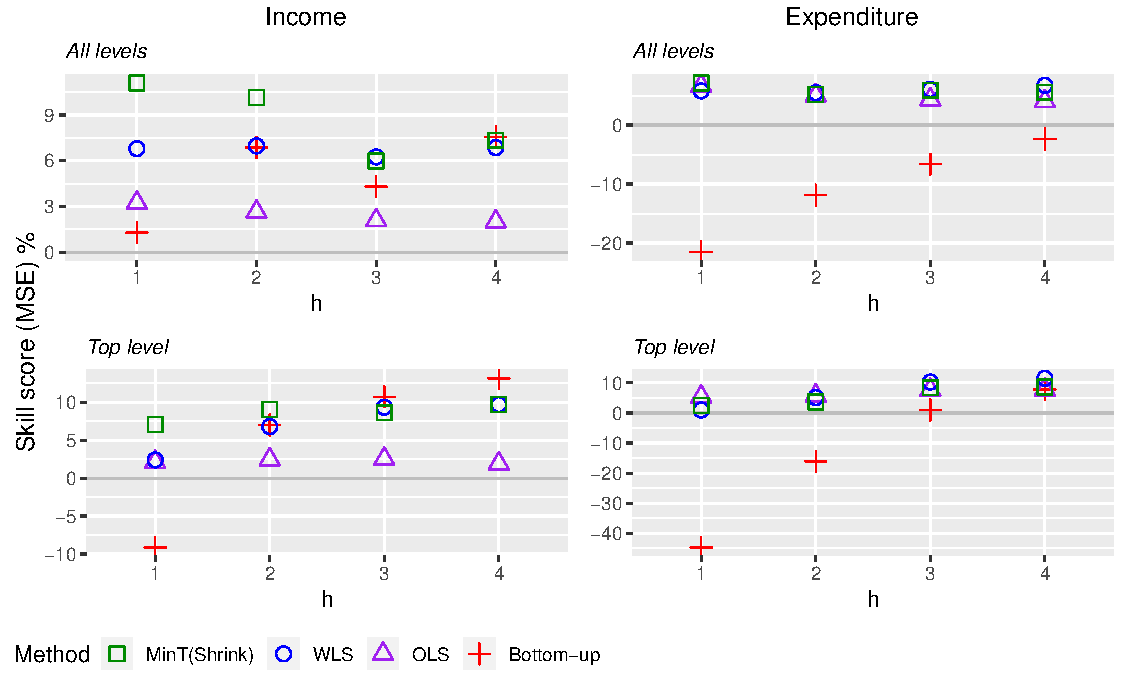
\includegraphics[scale=0.55]{Figs/Results/PointF_MSE_AllandToplevel.pdf}
	
	
\end{itemize}
\end{frame}


%------------------%

\begin{frame}{Reconciled Point forecasts - \textit{Results}}
\begin{itemize}[<+-| alert@+>]
	\item[] 
	\tiny
	\centering
	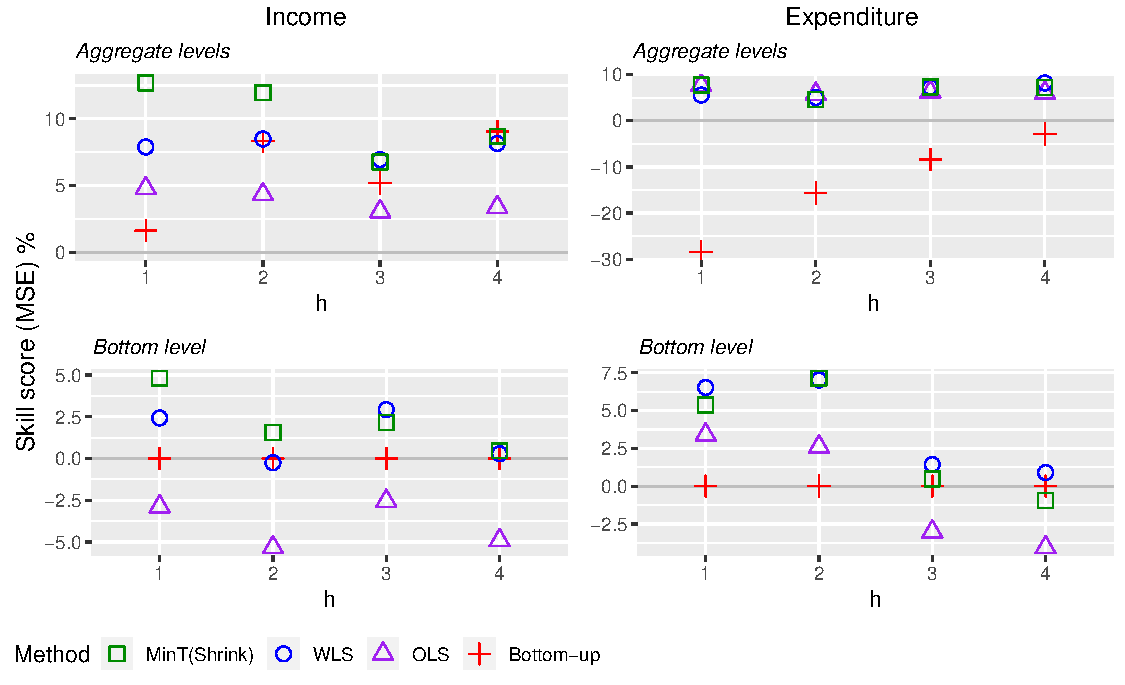
\includegraphics[scale=0.55]{Figs/Results/PointF_MSE_AggandDisagg.pdf}
	
	
\end{itemize}
\end{frame}


%------------------%

\begin{frame}{Probabilistic forecasts}
\begin{itemize}[<+-| alert@+>]
	\item Gaussian approach : 
	 \begin{equation*}
	 \color{Maroon}\mathscr{N}(\bm{SG}\bm{\hat{y}}_{T+h},~ \bm{SG}{\bm{W}}_{T+h}\bm{G}'\bm{S}')
	 \end{equation*}
		
	\item Non-parametric Bootstrap approach : 
	\begin{equation*}
	\color{Maroon} \tilde{\bm{\Upsilon}}_{T+h} = \bm{SG}\hat{\bm{\Upsilon}}'_{T+h}
	\end{equation*}
	where, $\hat{\bm{\Upsilon}}_{T+h} = (\hat{\bm{y}}^1_{T+h},...,\hat{\bm{y}}^B_{T+h})'$
\end{itemize}
\end{frame}


%------------------%

\begin{frame}{Reconciled Probabilistic Forecasts}
\begin{itemize}[<+-| alert@+>]
	\item[] 
	\tiny
	\centering
	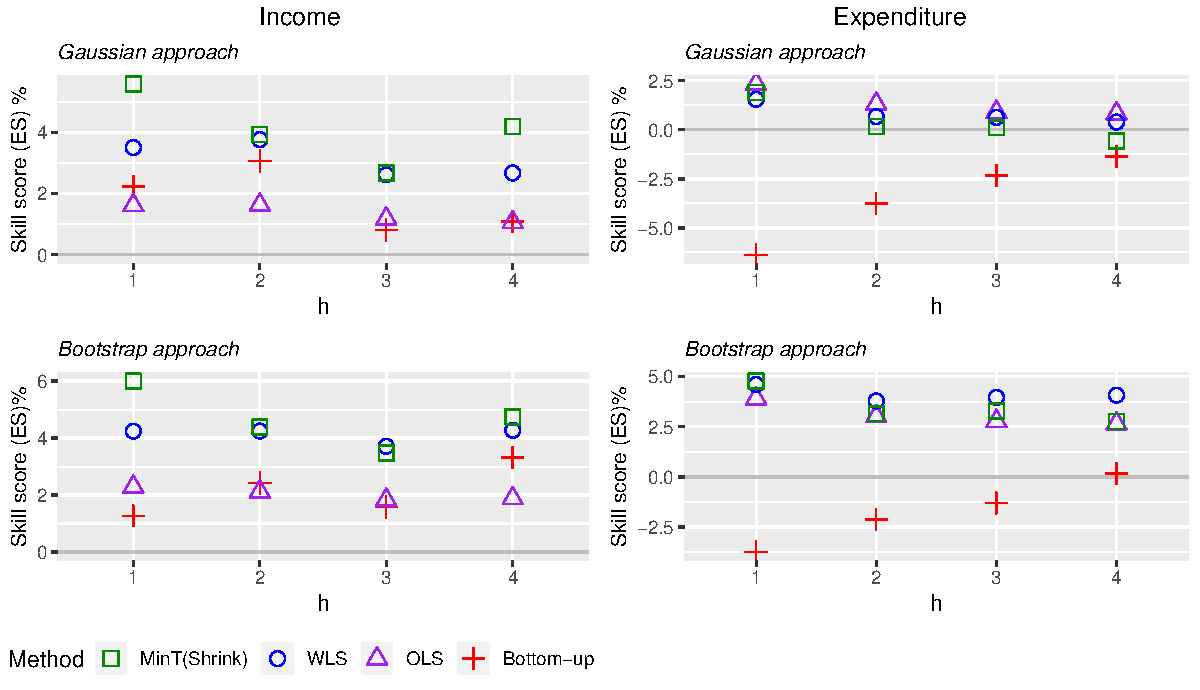
\includegraphics[scale=0.55]{Figs/Results/ProbF_MultivS_ES.pdf}
	
	
\end{itemize}
\end{frame}


%------------------%

\begin{frame}{Reconciled Probabilistic Forecasts}
\begin{itemize}[<+-| alert@+>]
	\item[] 
	\tiny
	\centering
	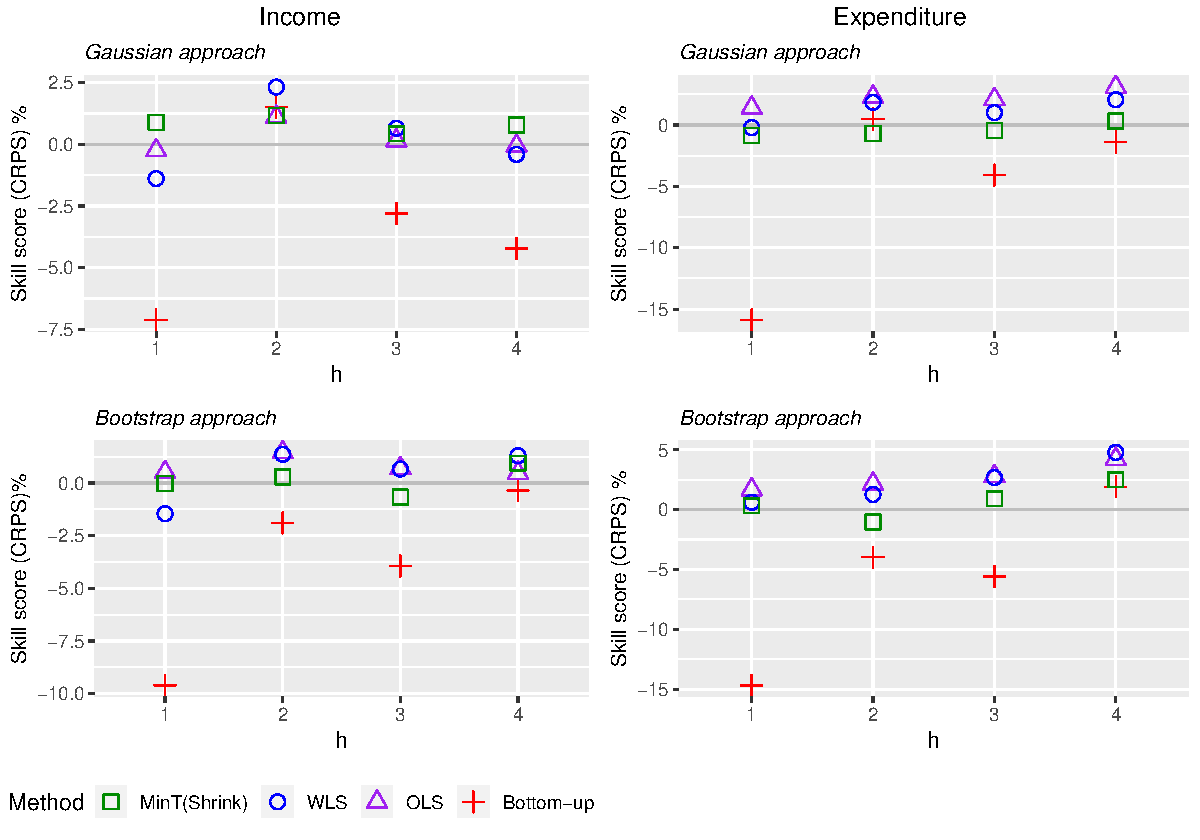
\includegraphics[scale=0.55]{Figs/Results/ProbF_UnivS.pdf}
	
	
\end{itemize}
\end{frame}


%------------------%



\section{Summary and time plan for completion}

\begin{frame}
\frametitle[]
%\frametitle{A first slide}

\begin{center}
\Huge Summary and time plan for completion
\end{center}
\end{frame}

\begin{frame}[noframenumbering]{Summary}
	\begin{itemize}[<+-| alert@+>]
		\item We define point and probabilistic forecast reconciliation in geometric terms.
		\item We propose a parametric approach for probabilistic forecast reconciliation. 
		
%		\item[]
%		\item Our definition holds for linear and non-linear reconciliation
%		\item[]
%		\item Linear reconciliation involves two steps
%		\item[] Step 1: Transform coordinates of incoherent probabilistic forecasts 
%		\item[] Step 2: Marginalize over the null space of the coherent subspace
%		\item[]
%		\item MinT not only produces optimal point forecasts, but also optimally reconcile Gaussian forecast densities
		\item We introduce a novel non-parametric bootstrap approach for producing reconciled probabilistic forecasts.
		\item[]
		\item Simulation study provides evidence that the optimal reconciliation with respect to energy score is equivalent to reconciling each sample path via MinT approach.
		\item[]
		\item We apply hierarchical forecast reconciliation methods to forecast Australian GDP in point as well as probabilistic framework.
		
	\end{itemize}
\end{frame}


\begin{frame}{Time plan for completion}
\begin{table}
	
	\centering \small
	\resizebox{\linewidth}{!}{
		\begin{tabular}{lllll }
			
			&\textbf{Thesis Chapter}& \textbf{Task description} & \textbf{Time duration} &  \textbf{Progress}\\  
			\toprule
			& & &  & \\
			1 and 2. & Introduction and Background Review &Writing the chapter.&September/2019 - October/2019 &40\% complete\\
			&&&&\\
			\midrule
			& & & & \\
			3. & Hierarchical forecast &  &&\\  
			& reconciliation & Bias correction and & May/2019 - July/2019 & 75\% Completed \\
			&in Geometric view& application&&\\
			
			&&&&\\
			\midrule
			&&&&\\
			4. & Probabilistic forecast &  &&\\  
			& reconciliation for & Completing the paper. & June/2019 - August/2019 & 90\% Completed \\
			& hierarchical time series &&&\\
			&&&&\\
			\midrule
			&&&&\\
			5. & Application & Forecasting Australian GDP & & 100\% Completed\\
			&&&&\\
			
			\bottomrule
		\end{tabular}
	}
\end{table}
\end{frame}
%
%
%
%%%%%%START%%%%%
%%--------------------------------------------
%
%
%%--------------------------------
%
%
\begin{frame}[noframenumbering,allowframebreaks]{References}
\printbibliography
\end{frame}
%
\begin{frame}[noframenumbering]
\frametitle[]
%\frametitle{A first slide}

\begin{center}
\Huge Thank You!!
\end{center}
\end{frame}

%\begin{frame}[noframenumbering]{Appendix}
%
%\begin{itemize}
%\item \hypertarget{OLS}{\beamerreturnbutton{A1}} \textbf{Optimal reconciliation approach}
%\begin{itemize}
%\item[$\bullet$] based on a regression, \\
%$\hat{\bm{y}}_{T+h} = \bm{S\beta}_{T+h} + \bm{\varepsilon}_{T+h}$
%\end{itemize}
%	\begin{block}{}
%$ \color{Maroon} OLS: \quad \bm{P} = (\bm{S}^T\bm{S})^{-1}\bm{S}^T$
%\end{block}
%\end{itemize}
%\end{frame}
%
%

%\begin{frame}[noframenumbering]{Appendix}
%\begin{itemize}[<+-| alert@+>]
%	\item[] \hypertarget{Prob_Gauss}{\beamerreturnbutton{A2}}
%	\item By substituting the Gaussian distribution function for $\hat{\bm{f}}(\cdot)$ in $\bm{f_B}(\cdot)$ we get, 
%	\begin{align*}
%	\bm{f_B}(\cdot)
%	& =
%	\frac{1}{(2\pi)^{\frac{n}{2}}\Big|\PQ\bm{{W}_{t+h}}\PQ'\Big|^{\frac{1}{2}}}
%	\exp \Big\{-\frac{1}{2} \begin{pmatrix}\tilde{\bm{b}}_{t+h} - \bm{P}\bm{\hat{y}}_{t+h}\\ \bm{t}_{t+h}- \bm{Q}\bm{\hat{y}}_{t+h}\end{pmatrix}' \\
%	& \Big[\PQ\bm{{W}_{t+h}}\PQ'\Big]^{-1}\begin{pmatrix}\tilde{\bm{b}}_{t+h} - \bm{P}\bm{\hat{y}}_{t+h}\\ \bm{t}_{t+h}- \bm{Q}\bm{\hat{y}}_{t+h}\end{pmatrix} \Big\}.
%	\end{align*}
%	where$$
%	(\bm{S} ~ \vdots~ \bm{R})^{-1} =
%	\begin{pmatrix}(\bm{R}'_\bot \bm{S})^{-1}\bm{R}'_\bot \\ \cdots \\ (\bm{S}'_\bot \bm{R})^{-1}\bm{S}'_\bot \end{pmatrix} =
%	\begin{pmatrix}
%	\bm{P} \\\bm{Q}
%	\end{pmatrix},
%	$$
%	and $\bm{P}=(\bm{R}'_\bot \bm{S})^{-1}\bm{R}'_\bot$ and $\bm{Q}=(\bm{S}'_\bot \bm{R})^{-1}\bm{S}'_\bot$.
%	
%\end{itemize}    
%
%\end{frame}

%------------------------%

\begin{frame}[noframenumbering]{Appendix: Probabilistic forecasts reconciliation assuming Gaussianity}\hypertarget{GaussianFramework}{\hyperlink{backtoGaussianFramework}{\beamerbutton{A1}}}
\begin{itemize}[<+-| alert@+>]
	\item Assuming Gaussianity, let an incoherent forecast distribution at time $T+h$ be given by
	$$\mathscr{N}(\hat{\bm{y}}_{T+h}, \bm{W}_{T+h}) \overset{d}{\leftrightarrow} \hat{\bm{f}}(.)$$ 
	where $\hat{\bm{y}}_{T+h}$ is the incoherent mean and ${\bm{W}}_{T+h} =E_{\bm{y}_{T+h}}[(\bm{y}_{T+h}-\hat{\bm{y}}_{T+h})(\bm{y}_{T+h}-\hat{\bm{y}}_{T+h})^T|\mathcal{I}_{T}]$ is incoherent variance 
	\item[]
	\item Gaussian densities are closed under affine transformation and marginalization
	\item From the linear transformation
	\begin{table}
		\centering \small
		
		$
		\bm{f_B}(\cdot)
		= \frac{\exp\left\{-\frac{1}{2}\Big((\bm{S} ~ \vdots~ \bm{R})\bth-\bm{\hat{y}}_{T+h}\Big)' \bm{W_{T+h}}^{-1}\Big((\bm{S} ~ \vdots~ \bm{R})\bth-\bm{\hat{y}}_{T+h}\Big)\right\}}{(2\pi)^{\frac{n}{2}}\Big|\bm{W}_{T+h}\Big|^{\frac{1}{2}}\Big|(\bm{S} ~ \vdots~ \bm{R})^{-1}\Big|}
		$\\
		
		
	\end{table}
	
	%	\begin{table}
	%		\small
	%		\centering %\setstretch{1.5}
	%		\begin{tabular}{l}
	%			
	%		\end{tabular}
	%	\end{table}
	
	
\end{itemize}    

\end{frame}

%------------------------


\begin{frame}[noframenumbering]{Appendix: Probabilistic forecasts reconciliation assuming Gaussianity}
\begin{itemize}[<+-| alert@+>]
\item Marginalizing over $\bm{t}_{T+h}$	 \hyperlink{Prob_Gauss}{\beamerbutton{A1}}
\begin{table}
	\small
	$$	
	\tilde{\bm{f}}_b(\tilde{\bm{b}}_{T+h})=\frac{\exp \Big\{-\frac{1}{2} (\tilde{\bm{b}}_{T+h} - \bm{G}\bm{\hat{y}}_{T+h})' (\bm{G}\bm{{W}_{T+h}}\bm{G}')^{-1}(\tilde{\bm{b}}_{T+h} - \bm{G}\bm{\hat{y}}_{T+h}) \Big\}}{(2\pi)^{\frac{n}{2}}\Big|\bm{G}\bm{{W}_{T+h}}\bm{G}'\Big|^{\frac{1}{2}}}
	$$	
\end{table}
\item This implies, $\tilde{\bm{b}}_{T+h} \sim \mathscr{N}(\bm{G}\bm{\hat{y}}_{T+h}, \bm{G}{\bm{W}}_{T+h}\bm{G}')$ where \color{Purple}$\bm{G} = (\bm{R}'_\bot \bm{S})^{-1}\bm{R}'_\bot$ 
\item Therefore the reconciled Gaussian distribution of the whole hierarchy is given by 
$$\color{Maroon}\tilde{\bm{f}}(\tilde{\bm{y}}_{t+h})=\tilde{\bm{f}}_b(\bm{S}\tilde{\bm{b}}_{T+h})\overset{d}{\leftrightarrow}\mathscr{N}(\bm{SP}\bm{\hat{y}}_{T+h},~ \bm{SP}{\bm{W}}_{T+h}\bm{G}'\bm{S}'),$$
where $\color{Purple}\bm{G} = (\bm{R}'_\bot \bm{S})^{-1}\bm{R}'_\bot$
\item[]
\item \textbf{\color{Maroon} Goal}: Solve for $\bm{G}$ by minimizing a \color{red} proper scoring rule
\end{itemize}    

\end{frame}

%--------------%


%------------------------

\begin{frame}[noframenumbering]{Appendix: Probabilistic forecasts reconciliation assuming Gaussianity}
\begin{itemize}[<+-| alert@+>]
\item We use the {\color{purple}Energy Score}, which is a proper scoring rule 
$$ES(\bm{\tilde{Y}_{T+h},y_{T+h}}) = E_{\bm{Y}_{T+h}}||\tilde{\bm{Y}}_{T+h}-\bm{y}_{T+h}||^\alpha - \frac{1}{2}E_{\bm{Y}_{T+h}}||\tilde{\bm{Y}}_{T+h}-\tilde{\bm{Y}}^*_{T+h}||^\alpha, $$ for $\alpha \in (0,2]$,\\
\item[] where $\tilde{\bm{Y}}_{T+h}$ and $\tilde{\bm{Y}}^*_{T+h}$ are independent random variables from $\mathcal{N}(\bm{SP}\hat{\bm{y}}_{T+h}, \bm{SP}{\bm{W}}_{T+h}\bm{P'S'})$.
\item[]
\item There is no closed form expression for $ES(\bm{\tilde{Y}_{T+h},y_{T+h}})$ for $\alpha \in (0,2)$ under the Gaussian predictive distribution
\item[]
\item However in the upper limit of $\alpha$, i.e. when $\alpha=2$,
$$ES(\bm{\tilde{Y}_{T+h},y_{T+h}})=||\bm{SP}\hat{\bm{y}}_{T+h}-\bm{y}_{T+h}||^2$$
\end{itemize}    

\end{frame}

%------------------------

\begin{frame}[noframenumbering]{Appendix: Probabilistic forecasts reconciliation assuming Gaussianity}
\begin{itemize}[<+-| alert@+>]
\item Then our objective function is
$$ \operatorname*{arg\,min}_{\bm{G}} Tr\{E_{\bm{y}_{T+h}}[(\bm{y}_{T+h}-\bm{SP}\hat{\bm{y}}_{T+h})(\bm{y}_{T+h}-\bm{SP}\hat{\bm{y}}_{T+h})^T|\mathcal{I}_{T}]\},$$ where $\bm{\mathcal{I}}_{T}=\{\bm{y}_1,....,\bm{y}_T\}$
\item Assuming unbiasedness for coherent forecasts
\begin{block}{}
$$ \argmin\limits_{\bm{G}} Tr \{\bm{SG{W}}_{T+h}\bm{G}^T\bm{S}^T\}$$
$$\text{Subject to} \quad \bm{SPS=S}$$
\end{block}

\item \citet{Wickramasuriya2018} have shown that a unique solution to this optimization problem attain at
$$\color{Maroon}  \bm{G} = (\bm{S}^T\bm{\bm{W}}_{T+h}^{-1}\bm{S})^{-1}\bm{S}^T\bm{\bm{W}}_{T+h}^{-1}.$$ 
\item Thus $\bm{R}'_\bot = \bm{S}'\bm{W}_{T+h}^{-1}$. This is referred to as {\color{red}MinT} solution
\end{itemize}    

\end{frame}

%------------------------
\begin{frame}[noframenumbering]{Appendix: Probabilistic forecasts in the Gaussian framework}
\begin{itemize}[<+-| alert@+>]
\item[] \color{Purple}$\bm{R}'_\bot = \bm{S}'\bm{W}_{T+h}^{-1}$
\item The optimally reconciled Gaussian forecast density is given by
\color{Maroon}$\mathcal{N}[\bm{S}(\bm{R}'_\bot \bm{S})^{-1}\bm{R}'_\bot\hat{\bm{y}}_{T+h}, \bm{S}(\bm{R}'_\bot \bm{S})^{-1}\bm{R}'_\bot{\bm{W}}_{T+h}\bm{R}_\bot(\bm{R}'_\bot \bm{S})^{-1}\bm{S'}]$, 

\item Different estimators of ${\bm{W}}_{T+h}$ yield different $\bm{R}'_\bot$ matrices 
\item[]
\item[]
\begin{center}
\begin{block}{}
\begin{table}
\small
\centering %\setstretch{1.5}
\begin{tabular}{lll}
	\toprule
	\textbf{Method} & \textbf{Estimate of $\bm{W}_{h}$} & \textbf{Estimate of $\bm{R}'_\bot$}      \\
	\midrule
	OLS             &
	$\bm{I}$  &
	$\bm{S}'$  \\
	MinT(Sample)    &
	$\bm{\hat{W}}_{T+1}^{sam}$ &
	$\bm{S}'(\bm{\hat{W}}_{T+1}^{sam})^{-1}$ \\
	MinT(Shrink)    &
	$\bm{\hat{W}}_{T+1}^{shr} = \tau\text{Diag}(\bm{\hat{W}}_{T+1}^{sam}) + (1-\tau)\bm{\hat{W}}_{T+1}^{sam}$\hyperlink{Shrinkage} {\beamerbutton{A2}} &
	$\bm{S}'(\bm{\hat{W}}_{T+1}^{shr})^{-1}$ \\
	MinT(WLS)       &
	$\bm{\hat{W}}_{T+1}^{wls} = \text{Diag}(\bm{\hat{W}}_{T+1}^{shr})$ &
	$\bm{S}'(\bm{\hat{W}}_{T+1}^{wls})^{-1}$ \\
	\bottomrule
\end{tabular}
\end{table}
\end{block}
\end{center}
\item[]
\item Predictive ability of the reconciled Gaussian densities from these methods will be evaluated in a simulation setting

\end{itemize}    
\end{frame}


\begin{frame}[noframenumbering]{Appendix: \textit{Probabilistic forecasts evaluation}}\hypertarget{ScoringRules}{\hyperlink{backtoScoringRule}{\beamerbutton{A2}}}
%{\beamerreturnbutton{A1}}
\begin{itemize}
	\item[]
	\begin{block}{}
		\begin{table}
			\small
			\centering %\setstretch{1.5}
			\resizebox{\linewidth}{!}{
				\begin{tabular}{lll}
					\textbf{Energy score}  & & \citep{Gneiting2008}\\
					$\text{eS}(\breve{\bm{Y}}_{T+h},\bm{y}_{T+h})$&=&
					$
					\E_{\breve{\bm{F}}}
					\|\breve{\bm{Y}}_{T+h}-\bm{y}_{T+h}\|^\alpha -
					\frac{1}{2}\E_{\breve{\bm{F}}}\|\breve{\bm{Y}}_{T+h}-\breve{\bm{Y}}^*_{T+h}\|^\alpha, \quad \alpha \in (0,2]$ \\
					&&\\
					%&& $\alpha \in (0,2]$\\ 
					\textbf{Log score}& & \citep{Gneiting2007}\\
					
					$\text{LS}(\breve{\bm{F}},\bm{y}_{T+h})$ & = & $-\log {\breve{\bm{f}}(\bm{y}_{T+h})}$\\
					&&\\
					\textbf{Variogram score} & & \citep{SCHEUERER2015}\\
					
					$\text{VS}(\breve{\bm{F}}, \bm{y}_{T+h})$ &=&
					$\sum\limits_{i=1}^{n}
					\sum\limits_{j=1}^{n}
					w_{ij}\Big(|y_{T+h,i} - y_{T+h,j}|^p-\E_{\breve{\bm{F}}}|\breve{Y}_{T+h,i}-\breve{Y}_{T+h,j}|^p\Big)^2$\\ 
					
					&&\\
					\textbf{CRPS} & & \citep{Gneiting2007}\\
					
					$\text{CRPS}(\breve{F}_i,y_{T+h,i})$ &=&
					$\E_{\breve{F}_i}|\breve{Y}_{T+h,i}-y_{T+h,i}| - \frac{1}{2}\E_{\breve{F}_i}|\breve{Y}_{T+h,i}-\breve{Y}^*_{T+h,i}|$\\ 
					
					
				\end{tabular}
			}
		\end{table}
		
	\end{block}
	
	\begin{table}
		\small
		\centering %\setstretch{1.5}
		\begin{tabular}{lll}
			\toprule
			$\breve{\bm{Y}}_{T+h}$ and $\breve{\bm{Y}}^*_{T+h}$ & : & Independent random vectors from the coherent \\
			& & forecast distribution $\breve{\bm{F}}$.\\
			$\bm{y}_{T+h}$ & : &Vector of realizations. \\
			$\breve{Y}_{T+h,i}$ and $\breve{Y}_{T+h,j}$ & : & $i$th and $j$th components of the vector $\breve{\bm{Y}}_{T+h}$ \\
			$w_{ij}$ & : & Non-negative weights\\
			\bottomrule
		\end{tabular}
	\end{table}
	
\end{itemize}

\end{frame}

%-------------------------

\begin{frame}[noframenumbering]{Appendix}
\begin{itemize}
	\item \hypertarget{Shrinkage}{\beamerreturnbutton{A2}} Shrinkage estimator for 1-step ahead base forecast errors
	$$
	\hat{\bm{\Sigma}}_{T+1}^{shr} = \tau\hat{\bm{\Sigma}}_{T+1}^D + (1-\tau)\hat{\bm{\Sigma}}_{T+1},
	$$
	where $\hat{\bm{\Sigma}}_{T+1}^D$ is the diagonal matrix comprising diagonal entries of $\hat{\bm{\Sigma}}_{T+1}$ and $$\tau = \frac{\sum_{i \ne j}\hat{Var}(\hat{r}_{ij})}{\sum_{i \ne j}\hat{r}_{ij}^2}$$ is a shrinkage parameter. $\hat{r}_{ij}$ is the $ij$-th element of sample correlation matrix.  In this estimation, the off-diagonal elements of 1-step ahead sample covariance matrix will be shrunk to zero depending on the sparsity.
	
\end{itemize}
\end{frame}

%-----------------%
\begin{frame}[noframenumbering]{Monte-Carlo simulation}
\begin{itemize}[<+-| alert@+>]
	\item \textbf{Data generating process}\hypertarget{Simulation}{\beamerreturnbutton{A3}}
	\begin{columns}
		\column{0.25\linewidth}
		\centering
		\begin{figure}
			\begin{center}
				\leaf{AA} \leaf{AB} 
				\branch{2}{A}
				\leaf{BA} \leaf{BB}
				\branch{2}{B}
				\branch{2}{Tot}
				\qobitree
			\end{center}
		\end{figure}
		
		\column{0.70\linewidth}
		\begin{itemize}[<+-| alert@+>]
			\item $\{w_{AA,t},w_{AB,t},w_{BA,t},w_{BB,t}\} \sim ARIMA(p,d,q)$ 	
			\item	$p \in \{1,2\}$ and $d \in \{0,1\}$
			\item $\{\epsilon_{AA,t},\epsilon_{AB,t},\epsilon_{BA,t},\epsilon_{BB,t}\} \sim \mathcal{N}(\bm{0}, \bm{\Sigma})$
			\item Parameters for $AR$ and $MA$ components were randomly and uniformly generated from $[0.3,0.5]$ and $[0.3,0.7]$ respectively
			
		\end{itemize}	
	\end{columns} 
	
	\item[]
	\item $\bm{y}_t$ are then generated as follows
	\item[]\begin{table}
		\small
		\centering %\setstretch{1.5}
		\resizebox{\linewidth}{!}{
			\begin{tabular}{lll}
				\toprule
				\textbf{Bottom level} & \textbf{Aggregate level 1} & \textbf{Total}      \\
				\midrule
				$y_{AA,t} = w_{AA,t} + u_t - 0.5v_t$ & $y_{A,t} = w_{AA,t} + w_{AB,t} - v_t$ & $y_{Tot,t} = w_{AA,t} + w_{AB,t} + w_{BA,t} + w_{BB,t}$\\
				$y_{AB,t} = w_{AB,t} - u_t - 0.5v_t$ & $y_{B,t} = w_{BA,t} + w_{BB,t} + v_t$ &\\
				$y_{BA,t} = w_{BA,t} + u_t + 0.5v_t$ & &\\
				$y_{BB,t} = w_{BB,t} - u_t + 0.5v_t$ & &\\
				\bottomrule
			\end{tabular}
		}
	\end{table}
	
	
\end{itemize} 
\end{frame}
%

\begin{frame}[noframenumbering]{Monte-Carlo simulation \textit{Cont..}}
\begin{itemize}[<+-| alert@+>]
\item To get less noisier series at aggregate levels, we choose $\bm{\Sigma}, \sigma^2_u$ and $\sigma^2_v$ such that,
\begin{table}
	\small
	\centering %\setstretch{1.5}
	\resizebox{\linewidth}{!}{
		\begin{tabular}{l}
			$
			\text{Var}(\epsilon_{AA,t}+\epsilon_{AB,t}+\epsilon_{BA,t}+\epsilon_{BB,t}) \le \text{Var}(\epsilon_{AA,t}+\epsilon_{AB,t}-v_t) \le \text{Var}(\epsilon_{AA,t}+u_t-0.5v_t),
			$\\
		\end{tabular}
	}
\end{table}

\item Thus we choose,
$\bm{\Sigma} =
\begin{pmatrix}
5.0 & 3.1 & 0.6 & 0.4 \\
3.1 & 4.0 & 0.9 & 1.4 \\
0.6 & 0.9 & 2.0 & 1.8 \\
0.4 & 1.4 & 1.8 & 3.0 \\
\end{pmatrix}$,
$\sigma^2_u = 19$ and $\sigma^2_u = 18$.


\end{itemize} 
\end{frame}
%

\begin{frame}[noframenumbering]{Sample version of the scoring rules}
\begin{itemize}[<+-| alert@+>]
	
	\item For a possible finite sample of size $B$ from the multivariate forecast density $\breve{\bm{F}}$, the variogram score is defined as,
	\begin{table}
	\small
	$\text{VS}(\breve{\bm{F}}, \bm{y}_{T+h}) = \displaystyle\sum_{i=1}^{n}\displaystyle\sum_{j=1}^{n}w_{ij}\left(|y_{T+h,i} - y_{T+h,j}|^p - \frac{1}{B} \displaystyle\sum_{k=1}^{B} |\breve{Y}^k_{T+h,i}-\breve{Y}^k_{T+h,j}|^p\right)^2$
	\end{table}
		
	
\end{itemize} 
\end{frame}
%


\end{document}
